%%
%% This is file `sample-authordraft.tex',
%% generated with the docstrip utility.
%%
%% The original source files were:
%%
%% samples.dtx  (with options: `authordraft')
%% 
%% IMPORTANT NOTICE:
%% 
%% For the copyright see the source file.
%% 
%% Any modified versions of this file must be renamed
%% with new filenames distinct from sample-authordraft.tex.
%% 
%% For distribution of the original source see the terms
%% for copying and modification in the file samples.dtx.
%% 
%% This generated file may be distributed as long as the
%% original source files, as listed above, are part of the
%% same distribution. (The sources need not necessarily be
%% in the same archive or directory.)
%%
%% Commands for TeXCount
%TC:macro \cite [option:text,text]
%TC:macro \citep [option:text,text]
%TC:macro \citet [option:text,text]
%TC:envir table 0 1
%TC:envir table* 0 1
%TC:envir tabular [ignore] word
%TC:envir displaymath 0 word
%TC:envir math 0 word
%TC:envir comment 0 0
%%
%%
%% The first command in your LaTeX source must be the \documentclass command.
\documentclass[sigconf, anonymous, review]{acmart}
\acmSubmissionID{967}
\usepackage[mathscr]{euscript}
%% NOTE that a single column version may required for 
%% submission and peer review. This can be done by changing
%% the \doucmentclass[...]{acmart} in this template to 
%% \documentclass[manuscript,screen]{acmart}
%%
\usepackage{algpseudocode}
\usepackage{algorithm,colortbl,xcolor}
\definecolor{Gray}{gray}{0.85}
%% To ensure 100% compatibility, please check the white list of
%% approved LaTeX packages to be used with the Master Article Template at
%% https://www.acm.org/publications/taps/whitelist-of-latex-packages 
%% before creating your document. The white list page provides 
%% information on how to submit additional LaTeX packages for 
%% review and adoption.
%% Fonts used in the template cannot be substituted; margin 
%% adjustments are not allowed.

%%
%% \BibTeX command to typeset BibTeX logo in the docs
\AtBeginDocument{%
  \providecommand\BibTeX{{%
    \normalfont B\kern-0.5em{\scshape i\kern-0.25em b}\kern-0.8em\TeX}}}

%% Rights management information.  This information is sent to you
%% when you complete the rights form.  These commands have SAMPLE
%% values in them; it is your responsibility as an author to replace
%% the commands and values with those provided to you when you
%% complete the rights form.
%\setcopyright{acmcopyright}
%\copyrightyear{2018}
%\acmYear{2018}
%\acmDOI{XXXXXXX.XXXXXXX}

%% These commands are for a PROCEEDINGS abstract or paper.
%\acmConference[Conference acronym 'XX]{Make sure to enter the correct conference title from your rights confirmation emai}{June 03--05,2018}{Woodstock, NY}
%
%  Uncomment \acmBooktitle if th title of the proceedings is different
%  from ``Proceedings of ...''!
%
%\acmBooktitle{Woodstock '18: ACM Symposium on Neural Gaze Detection,
%  June 03--05, 2018, Woodstock, NY} 
%\acmPrice{15.00}
%\acmISBN{978-1-4503-XXXX-X/18/06}


%%
%% Submission ID.
%% Use this when submitting an article to a sponsored event. You'll
%% receive a unique submission ID from the organizers
%% of the event, and this ID should be used as the parameter to this command.
%%\acmSubmissionID{123-A56-BU3}

%%
%% For managing citations, it is recommended to use bibliography
%% files in BibTeX format.
%%
%% You can then either use BibTeX with the ACM-Reference-Format style,
%% or BibLaTeX with the acmnumeric or acmauthoryear sytles, that include
%% support for advanced citation of software artefact from the
%% biblatex-software package, also separately available on CTAN.
%%
%% Look at the sample-*-biblatex.tex files for templates showcasing
%% the biblatex styles.
%%

%%
%% For managing citations, it is recommended to use bibliography
%% files in BibTeX format.
%%
%% You can then either use BibTeX with the ACM-Reference-Format style,
%% or BibLaTeX with the acmnumeric or acmauthoryear sytles, that include
%% support for advanced citation of software artefact from the
%% biblatex-software package, also separately available on CTAN.
%%
%% Look at the sample-*-biblatex.tex files for templates showcasing
%% the biblatex styles.
%%

%%
%% The majority of ACM publications use numbered citations and
%% references.  The command \citestyle{authoryear} switches to the
%% "author year" style.
%%
%% If you are preparing content for an event
%% sponsored by ACM SIGGRAPH, you must use the "author year" style of
%% citations and references.
%% Uncommenting
%% the next command will enable that style.
%%\citestyle{acmauthoryear}

%%
%% end of the preamble, start of the body of the document source.
\begin{document}

%%
%% The "title" command has an optional parameter,
%% allowing the author to define a "short title" to be used in page headers.
\title{Group Testing for Accurate and Efficient Nearest Neighbor Search: An Adaptive Binary Splitting Approach}

%%
%% The "author" command and its associated commands are used to define
%% the authors and their affiliations.
%% Of note is the shared affiliation of the first two authors, and the
%% "authornote" and "authornotemark" commands
%% used to denote shared contribution to the research.
\author{Ben Trovato}
\authornote{Both authors contributed equally to this research.}
\email{trovato@corporation.com}
\orcid{1234-5678-9012}
\author{G.K.M. Tobin}
\authornotemark[1]
\email{webmaster@marysville-ohio.com}
\affiliation{%
  \institution{Institute for Clarity in Documentation}
  \streetaddress{P.O. Box 1212}
  \city{Dublin}
  \state{Ohio}
  \country{USA}
  \postcode{43017-6221}
}

\author{Lars Th{\o}rv{\"a}ld}
\affiliation{%
  \institution{The Th{\o}rv{\"a}ld Group}
  \streetaddress{1 Th{\o}rv{\"a}ld Circle}
  \city{Hekla}
  \country{Iceland}}
\email{larst@affiliation.org}

\author{Valerie B\'eranger}
\affiliation{%
  \institution{Inria Paris-Rocquencourt}
  \city{Rocquencourt}
  \country{France}
}

\author{Aparna Patel}
\affiliation{%
 \institution{Rajiv Gandhi University}
 \streetaddress{Rono-Hills}
 \city{Doimukh}
 \state{Arunachal Pradesh}
 \country{India}}

\author{Huifen Chan}
\affiliation{%
  \institution{Tsinghua University}
  \streetaddress{30 Shuangqing Rd}
  \city{Haidian Qu}
  \state{Beijing Shi}
  \country{China}}

\author{Charles Palmer}
\affiliation{%
  \institution{Palmer Research Laboratories}
  \streetaddress{8600 Datapoint Drive}
  \city{San Antonio}
  \state{Texas}
  \country{USA}
  \postcode{78229}}
\email{cpalmer@prl.com}

\author{John Smith}
\affiliation{%
  \institution{The Th{\o}rv{\"a}ld Group}
  \streetaddress{1 Th{\o}rv{\"a}ld Circle}
  \city{Hekla}
  \country{Iceland}}
\email{jsmith@affiliation.org}

\author{Julius P. Kumquat}
\affiliation{%
  \institution{The Kumquat Consortium}
  \city{New York}
  \country{USA}}
\email{jpkumquat@consortium.net}

%%
%% By default, the full list of authors will be used in the page
%% headers. Often, this list is too long, and will overlap
%% other information printed in the page headers. This command allows
%% the author to define a more concise list
%% of authors' names for this purpose.
\renewcommand{\shortauthors}{Trovato and Tobin, et al.}

%%
%% The abstract is a short summary of the work to be presented in the
%% article.
\begin{abstract}
This work presents an adaptive group testing framework for the high dimensional nearest neighbor search problem. The proposed method detects high-similarity vectors from an extensive collection of high-dimensional vectors, where each vector represents an image descriptor or any other feature set used for description. Our method marks each and every item in the collection as neighbor or non-neighbor on the basis of cosine distance in an efficient manner without exhaustive search. Like other methods in the domain of large scale retrieval, our approach exploits the assumption that most of the items in the collection are unrelated to the query. Unlike other methods, it does not assume a large difference between the cosine similarity of the query vector with the least related neighbor and that with the least unrelated non-neighbor. Following the procedure of binary splitting, a multi-stage adaptive group testing algorithm, we split the set of items to be searched into half at each step, and perform dot product tests on smaller and smaller subsets, many of which we are able to prune away. We experimentally show that our method achieves a speed-up over exhaustive search by a factor of more than ten with an accuracy same as that of exhaustive search, on a variety of large datasets. Assuming an exponential distribution of cosine distances between a query vector and the vectors in the collection, we also demonstrate a theoretical analysis of the expected number of distance computations per query. 
In our method, all required data structures are created purely offline. Moreover, our method does not impose any strong assumptions related to the number of true near neighbors, and does not require any parameter tuning. 
\end{abstract}

%%
%% The code below is generated by the tool at http://dl.acm.org/ccs.cfm.
%% Please copy and paste the code instead of the example below.
%%

%%
%% Keywords. The author(s) should pick words that accurately describe
%% the work being presented. Separate the keywords with commas.
\keywords{nearest neighbor search, group testing, adaptive group testing, compressed sensing, binary splitting}

%% A "teaser" image appears between the author and affiliation
%% information and the body of the document, and typically spans the
%% page.


% \begin{teaserfigure}
%   \includegraphics[width=\textwidth]{sampleteaser}
%   \caption{Seattle Mariners at Spring Training, 2010.}
%   \Description{Enjoying the baseball game from the third-base
%   seats. Ichiro Suzuki preparing to bat.}
%   \label{fig:teaser}
% \end{teaserfigure}

%%
%% This command processes the author and affiliation and title
%% information and builds the first part of the formatted document.
\maketitle

\section{Introduction}
Nearest neighbor (NN) search is a fundamental problem in machine learning, computer vision, image analysis, recommender systems and many areas of multimedia. Consider a collection $\mathcal{D}$ of $N$ vectors given as $\{\boldsymbol{f_1}, \boldsymbol{f_2}, \cdots, \boldsymbol{f_N}\}$ where each $\boldsymbol{f_i} \in \mathbb{R}^d$. Given a query vector $\boldsymbol{q} \in \mathbb{R}^d$, our aim is to determine all those 
vectors in $\mathcal{D}$ such that $\textrm{sim}(\boldsymbol{q},\boldsymbol{f_i}) \geq \rho$, where $\rho$ denotes some similarity threshold and $\textrm{sim}(.,.)$ denotes some similarity measure. This is called a similarity measure based NN query. Another variant is the $K$ nearest neighbor (KNN) search where the aim is to find the $K$ most similar neighbors to $\boldsymbol{q}$. 

There exists a large body of literature on approximate NN search in higher dimensions. One of the major contributions in this area is called locality sensitive hashing (LSH) \cite{Indyk1998}. In LSH, an LSH function is used to partition the dataset into buckets in such a manner that the similarity between vectors belonging to one and the same bucket is high. Given a query vector, one first determines which bucket it belongs to, and then distance measures between the query vector and each member of the bucket are computed. The LSH family of algorithms consists of many variants such as those involving multiple buckets per query vector, data-driven or machine learning based construction of LSH functions \cite{Andoni2015,Dong2019}, and count-based methods which count the number of LSH collisions \cite{Lv2007}. In general, LSH based methods are difficult to implement for very high dimensions owing to the curse of dimensionality in constructing effective hash tables. Dimensionality reduction algorithms can mitigate this issue to some extent, but they are themselves expensive to implement and incur some inevitable data loss. In work such as \cite{Ram2019,Muja2014}, different randomized variants of KD-trees or priority search K-means trees are used for efficient approximate NN search in high dimensions. 

\textbf{Group Testing:} In this work, we present a group testing (GT) based approach for the NN problem. Consider $N$ items $\{x_i\}_{i=1}^N$ (also called `samples' in many references), out of which only a small number $s \ll N$ are defective. We consider the $i$th item to be defective if $x_i = 1$ and non-defective if $x_i = 0$. GT involves testing a certain number of `pools' ($m \ll N$) to identify the defective items from the $N$ ones. Each pool is created by mixing together or combining subsets of the $N$ items. Thus the $j$th pool ($j \in [m]$) is represented as follows:
\begin{equation}
y_j = \vee_{i=1}^N A_{ji} x_i,   
\end{equation}
where $\vee$ stands for bit-wise OR, and $\boldsymbol{A} \in \{0,1\}^{m \times N}$ is a binary pooling matrix where $A_{ji} = 1$ if the $i$th item participates in the $j$th pool and 0 otherwise. 

GT has a rich literature dating back to the seminal work of Dorfman \cite{Dorfman1943} who proposed a popular two-round testing strategy. In the first round, some $N/K$ pools, each consisting of $K$ items, are tested. The items that participated in pools that test negative (that is, pools that are deemed to contain no defective item) are declared non-defective, whereas all items that participated in the positive pools are tested individually in the second round. This method is popularly called Dorfman's method. Theoretical analysis shows that for $s \ll N$, this method requires much fewer than $N$ tests in the worst case. This algorithm was extended to some $r$ rounds in \cite{Li1962}, where positive groups are further divided into smaller groups, and individual testing is performed only in the $r$th round. The methods in \cite{Dorfman1943, Li1962} are said to be \textbf{adaptive} in nature, as the results of one round are given as input to the next one. The GT literature also contains a large number of \textbf{non-adaptive} algorithms that make predictions in a single round.  A popular algorithm is called \textsc{Comp} or combinatorial orthogonal matching pursuit, which declares all items participating in a negative pool to be negative, and all the rest to be positive \cite{Aldridge2019}. Many variants of \textsc{Comp} such as Noisy \textsc{Comp} (\textsc{NComp}) or Definite Defectives (\textsc{Dd}) are also popular. A popular class of non-adaptive GT algorithms draw heavily from the compressed sensing (CS) literature \cite{Candes2008}. Such algorithms can consider quantitative information for each $\{x_i\}_{i=1}^N$ so that each $x_i \in \mathbb{R}$, and every pool $y_j$ also gives a real-valued result. The pooling matrix remains binary, and we have the following relation:
\begin{equation}
\forall j \in [m], y_j  = \sum_{i=1}^N A_{ji} x_i. 
\end{equation}
Given $\{y_j\}_{j=1}^m$ and $\boldsymbol{A}$, the unknown vector $\boldsymbol{x}$ can be recovered using efficient convex optimization methods such as the \textsc{Lasso} given as follows: 
\begin{equation}
\boldsymbol{\hat{x}} = \textrm{Argmin}_{\boldsymbol{x}} \|\boldsymbol{y}-\boldsymbol{Ax}\|^2_2 + \lambda \|\boldsymbol{x}\|_1, 
\end{equation}
where $\lambda$ is a regularization parameter \cite{Hastie2015}. As proved in \cite{Hastie2015, Davenport2012}, the \textsc{Lasso} estimator produces provably accurate estimates of $\boldsymbol{x}$ given a sufficient number of measurements (or pools) in $\boldsymbol{y}$ and a carefully designed matrix $\boldsymbol{A}$. 

\textbf{Overview of our work:} GT algorithms have been applied to the NN search problem in recent times in papers such as \cite{Shi2014, Iscen2018, Engels2021}. However in these papers, the nearest neighbor queries are of an \emph{approximate} nature, i.e. the results may contain a number of vectors which are not near neighbors of the query vector $\boldsymbol{q}$, and/or may miss some genuine near neighbors. On the other hand, we focus on \emph{accurate} query results with good computational efficiency in practice. Our approach is based on an adaptive GT approach called binary splitting. Like existing GT based algorithms such as \cite{Shi2014, Iscen2018, Engels2021}, our approach is also based on the assumption that in high-dimensional NN search, most vectors in the collection $\mathcal{D}$ are dissimilar to a query vector $\boldsymbol{q}$, and very few vectors qualify as near neighbors. Our algorithm is intuitive, very simple to implement, and shows excellent results in practice. 

\textbf{Organization of the paper:} The core method is presented in Sec.~\ref{sec:method}. We present detailed analytical comparisons with existing GT-based techniques for NN search in Sec.~\ref{sec:comparison}. Experimental results are presented in Sec.~\ref{sec:results}. A theoretical analysis of our approach is presented in Sec.~\ref{sec:theoretical_analysis}. We conclude in Sec.~\ref{sec:conclusion}.

\section{Description of Method}
\label{sec:method}
In our technique, a pool of high-dimensional vectors is created by simply adding together the participating vectors, which may for example be (vectorized) images or features extracted from them. Consider a query vector $\boldsymbol{q} \in \mathbb{R}^d$ and the collection $\mathcal{D}$ consisting of $\{\boldsymbol{f_1}, \boldsymbol{f_2},\cdots,\boldsymbol{f_N}\}$ where each $\boldsymbol{f_i} \in \mathbb{R}^d$. Throughout this paper, we consider the similarity measure $\textrm{sim}(\boldsymbol{q}, \boldsymbol{f_i}) \triangleq \boldsymbol{q}^t \boldsymbol{f_i}$. For simplicity, we consider the query vector $\boldsymbol{q}$ as well as the vectors in the collection to be element-wise non-negative. This constraint is satisfied by image or speech data. We also consider that the vectors in question have unit magnitude, without any loss of generality. Due to this, $\boldsymbol{q}^t \boldsymbol{f_i}$ acts as a cosine similarity measure. 
Our aim is to retrieve all `defective' members of $\mathcal{D}$, i.e. members $\boldsymbol{f_i}$ for which $\boldsymbol{q}^t \boldsymbol{f_i} \geq \rho$, where $\rho$ is some pre-specified threshold. With this aim in mind, we aim to efficiently prune away any vector $\boldsymbol{f_i}$ from $\mathcal{D}$ for which it is impossible to have $\boldsymbol{q}^t \boldsymbol{f_i} \geq \rho$. 

Pooling proves to be beneficial for this purpose: Consider the toy example of a pool $\boldsymbol{y} = \boldsymbol{f_1} + \boldsymbol{f_2} + \boldsymbol{f_3} + \boldsymbol{f_4}$. If $\boldsymbol{q}^t \boldsymbol{y} < \rho$ (i.e. the pooled result is negative), then one can clearly conclude that $\boldsymbol{q}^t \boldsymbol{f_i} < \rho$ for each $i \in \{1,2,3,4\}$. However if  $\boldsymbol{q}^t \boldsymbol{y} \geq \rho$, i.e. it yields a positive result, then we need to do further work to identify the defective members (if any). For this, we split the original pool and create two pools $\boldsymbol{y_1}$ and $\boldsymbol{y_2}$, each with approximately half the number of members of the original pool. We recursively compute $\boldsymbol{q}^t \boldsymbol{y_2}$, and then obtain $\boldsymbol{q}^t \boldsymbol{y_1} = \boldsymbol{q}^t \boldsymbol{y} - \boldsymbol{q}^t \boldsymbol{y_2}$ (where both dot products on the right hand side have already been computed earlier and hence $\boldsymbol{q}^t \boldsymbol{y_1}$ is directly obtained from the difference between them). We then proceed in a similar fashion for both branches. 

We now consider the case of searching within the entire collection $\mathcal{D}$ defined earlier. We initiate this recursive process with a pool $\boldsymbol{y_0}$ that is obtained from the summation of all $N$ vectors. If $\boldsymbol{y_0}$ yields 
a positive result, we test the query vector with two pools: $\boldsymbol{y_{11}}$ obtained from a summation of vectors $\boldsymbol{f_1}$ through to $\boldsymbol{f_{\lfloor N/2 \rfloor}}$, and $\boldsymbol{y_{12}}$ obtained from a summation of vectors $\boldsymbol{f_{\lfloor N/2 \rfloor+1}}$ through to $\boldsymbol{f_N}$. If $\boldsymbol{y_{11}}$ tests negative, then all its members are declared negative and no further tests are required on its members, which greatly reduces the total number of tests. If $\boldsymbol{y_{11}}$ tests positive, then it is split into two pools 
$\boldsymbol{y_{21}}, \boldsymbol{y_{22}}$ with roughly equal number of members. Tests are carried out further on these two pools recursively. The same treatment is accorded to $\boldsymbol{y_{12}}$, which would be split into pools $\boldsymbol{y_{23}}, \boldsymbol{y_{24}}$ if it were to test positive. This recursive process stops when the pools obtained after splitting contain just a single vector each, in which case each such single vector is tested against $\boldsymbol{q}$. Clearly, the depth of this recursive process is $\lceil \log_2 N \rceil$ given $N$ vectors in the collection $\mathcal{D}$. This procedure is called \textbf{binary splitting}, and it is a multi-round adaptive group testing approach, applied here to NN search. 

For efficiency of implementation, it is important to be able to create the different pools such as $\boldsymbol{y_0}, \boldsymbol{y_{11}}, \boldsymbol{y_{12}}, \boldsymbol{y_{21}}, \boldsymbol{y_{22}}, \boldsymbol{y_{23}}, \boldsymbol{y_{24}}$, etc., efficiently. For this purpose, we maintain cumulative sums of the following form in memory:
\begin{eqnarray}
\boldsymbol{\widetilde{f}_1} = \boldsymbol{f_1}, 
\boldsymbol{\widetilde{f}_2} = \boldsymbol{\widetilde{f}_1} + \boldsymbol{f_2}, 
\boldsymbol{\widetilde{f}_3} = \boldsymbol{\widetilde{f}_2} + \boldsymbol{f_3}, \nonumber \\
...\nonumber\\
\boldsymbol{\widetilde{f}_N} = \boldsymbol{\widetilde{f}_{N-1}} + \boldsymbol{f_N}. 
\label{eq:cumsums}
\end{eqnarray}
The cumulative sums are useful for efficient creation of various pools. They are created purely \emph{offline}, independent of any query vector. The pools are created using simple vector difference operations, given these cumulative sums. For example, notice that $\boldsymbol{y_0} = \boldsymbol{\widetilde{f}_N}, \boldsymbol{y_{11}} = \boldsymbol{\widetilde{f}_{\lfloor N/2 \rfloor}}$ and $\boldsymbol{y_{12}} = \boldsymbol{\widetilde{f}_N} - \boldsymbol{\widetilde{f}_{\lfloor N/2 \rfloor}}$. 

The overall binary splitting procedure is summarized in Alg.~\ref{alg:binsplt}. For the sake of greater efficiency, it is implemented non-recursively using a simple stack data structure. 

\begin{algorithm}
\caption{Iterative Binary Splitting}\label{alg:binsplt}
\begin{algorithmic}[1]
\State $Fs \gets [\boldsymbol{\widetilde{f}_1}, \boldsymbol{\widetilde{f}_2},...,\boldsymbol{\widetilde{f}_N}]$
\State $S \gets$ stack for storing\ triples $\{si, ei, sim\}$ where $si = $ start index, $ei = $ end index, $sim =$ similarity value.  
\State $Flg \gets$ array of size $N$ flags, all\ 0's initially ($0 =$ non-neighbor, $1 =$ neighbor of query vector $\boldsymbol{q}$)
\State $push\ \{1, N, \boldsymbol{q}^t\boldsymbol{\widetilde{f}_N}\}$, i.e. $si = 1, ei = N$
\While{$S.size() \neq 0$} 
    \State $\{si, ei, sim\} \gets S.top()$; $S.pop()$
    \If{$sim \geq \rho$}
        \State $n \gets ei-si+1$
        \If{$n > 2$}
            \State $rsim \gets \boldsymbol{q}^t(\boldsymbol{\widetilde{f}_{ei}} - \boldsymbol{\widetilde{f}_{si+\lfloor n/2 \rfloor-1}})$ \Comment{testing right-half}
            \State $push\ \{si+\lfloor n/2 \rfloor, ei, rsim\}$; \Comment{push right branch onto stack}
            \State $push\ \{si, si+\lfloor n/2 \rfloor-1,sim-rsim\}$; \Comment{push left branch onto stack}
        \Else
            \If{$n = 2$}
                \State $rsim \gets \boldsymbol{q}^t(\boldsymbol{\widetilde{f}_{ei}} - \boldsymbol{\widetilde{f}_{si}})$
                \State \textbf{set} $Flg[ei] = 1$, \textbf{if} $rsim \geq \rho$
                \State \textbf{set} $Flg[si] = 1$, \textbf{if} $sim - rsim$ $\geq$ $\rho$
            \Else
                \State $Flg[si] = 1$ \Comment{Mark $si$ a neighbor}
            \EndIf
        \EndIf
    \EndIf
\EndWhile
\end{algorithmic}
\end{algorithm}

This binary splitting approach is quite different from Dorfman's algorithm \cite{Dorfman1943}, which performs individual testing in the second round. Our approach is more similar to Hwang's generalized binary splitting approach, a group testing procedure which was proposed in \cite{Hwang1972}. The same procedure is also succinctly described in \cite{gbs_wiki} and presented as Algorithm 1.1 in \cite{Aldridge2019}. However compared to Hwang's technique, our approach allows for creation of all pools either in a purely offline manner or with simple updates involving a single vector-subtraction operation (for example, $\boldsymbol{y_{12}} = \boldsymbol{\widetilde{f}_N} - \boldsymbol{\widetilde{f}_{\lfloor N/2 \rfloor}}$ in the earlier example). On the other hand, the method in \cite{Hwang1972} detects defectives one at a time, after going through the full recursion, consisting of $\log_2 N$ levels of recursion. Once a defective item is detected, it is discarded and all pools are created again. The entire set of $\log_2 N$ levels of recursion are again executed. This process is repeated until all defectives have been detected and discarded one at a time. In the context of high-dimensional NN search, the method from \cite{Hwang1972} is computationally inefficient in terms of creation of the pools. This is because if a vector at index $i$ is discarded, all cumulative sums from index $i+1$ to $N$ need to be updated. Such updates are not required in our method. We also emphasize that the techniques in \cite{Dorfman1943,Aldridge2019,Hwang1972,Li1962} have all been applied for binary group testing and not for NN search. 

The binary splitting procedure saves on a large number of tests because in high dimensional search, we observe that most vectors in $\mathcal{D}$ are dissimilar to a given query vector $\boldsymbol{q}$, as will be demonstrated in Sec.~\ref{sec:results}. After the first round where pool $\boldsymbol{y_0}$ is created, all other pools are essentially created randomly (since the initial arrangement of the vectors in $\mathcal{D}$ is random). As a result, across the different rounds, many pools test negative and are dropped out, especially in later rounds. In particular, we note that there is no loss of accuracy in this method, although we save on the number of tests by a factor more than ten on some large datasets (as will be shown in Sec.~\ref{sec:results}). 

\section{Comparison to other Group Testing Methods for NN Search}
\label{sec:comparison}
The oldest work on GT for NN search was presented in \cite{Shi2014}. In this method, the original data vectors are represented as a matrix $\boldsymbol{F} \in \mathbb{R}^{N \times d}$. The pools are represented as a matrix $\boldsymbol{Y} \in \mathbb{R}^{m \times d}$ obtained by pre-multiplying $\boldsymbol{F}$ by a randomly generated balanced binary matrix $\boldsymbol{A}$ of size $m \times N$ where $m < N$. In a balanced binary matrix, each column has exactly $c$ ones, and each row has exactly $r$ ones such that $cN = mr$. This ensures that each vector participates in $c$ pools and that each pool is obtained by adding $r$ vectors. Given a query vector $\boldsymbol{q}$, its similarity with the $j$th pool is computed, yielding a score $v_{yj} = \boldsymbol{q}^t \boldsymbol{Y^j}$, where $\boldsymbol{Y^j}$ is the $j$th group vector (and the $j$th row of $\boldsymbol{Y}$). This is repeated for every $j \in [m]$. Let $\mathcal{P}_i$ be the set of pools in which the $i$th vector, i.e. $\boldsymbol{f_i}$, belongs. Then, a likelihood score $L_i \triangleq \sum_{j \in \mathcal{P}_i} v_{yj}$ is computed for every vector. The vector from $\boldsymbol{F}$ with the largest likelihood score (denote this vector by $\boldsymbol{f_{k0}}$) is considered to be one of the nearest neighbors of $\boldsymbol{q}$. Next, the value $\boldsymbol{q}^t \boldsymbol{f_{k0}}$ is computed and the pool-level similarity scores for all pools containing  $\boldsymbol{f_{k0}}$ are updated to yield new scores of the form $v_{yj} = v_{yj} - \boldsymbol{q}^t \boldsymbol{f_{k0}}$. Thereafter, all likelihood scores are updated. This process is called back-propagation in \cite{Shi2014}. Again, the vector from $\boldsymbol{F}$ with the highest likelihood is identified and this procedure is repeated some $R$ times, and finally a sort operation is performed in order to rank them. In \cite{Shi2014}, it is argued that the time complexity of this procedure is $O( d (m + R))$. However, this is an approximate search method, and there is no guarantee that the $R$ neighbors thus derived will indeed be the nearest ones. As a result, a large number of false positives may be generated by this method. The choice of the number of pools is an important hyper-parameter, the optimal value of which can vary across datasets and query vectors, and there appears no data-driven procedure to select it at query time.

The work in \cite{Iscen2018} clusters the collection $\mathcal{D}$ into disjoint groups such that the members of a group are as orthogonal to each other as possible. As a result, the similarity measure $\boldsymbol{q}^t \boldsymbol{y_j}$ between $\boldsymbol{q}$ and a group vector $\boldsymbol{y_j}$ is almost completely dominated by the similarity between $\boldsymbol{q}$ and exactly one member of the group. A careful sparse coding and decoder correction step is also used, and the sparsity of the codes plays a key role in the speedup achieved by this method. However, this method is again an approximate method and heavily relies on the near-orthogonality of each group. The method also requires choice of several hyper-parameters for sparse coding, and a choice of an appropriate number of pools. These parameters can vary across datasets and query vectors, and there is no clear data-driven approach to select them at query time. 

The work in \cite{Engels2021} randomly distributes the collection $\mathcal{D}$ of $N$ vectors over some $B$ cells. This is independently repeated $R$ times, creating a grid of $B \times R$ cells. Within each cell, we have a collection of participating members $M_{r,b}$ and a corresponding group test $C_{r,b}$. The group test is essentially a binary classifier which determines whether $M_{r,b}$ contains at least one member which is similar to the query vector $\boldsymbol{q}$. This is an approximate query, with a true positive rate $p$ and false positive rate $q$. It is implemented via a distance-sensitive bloom filter \cite{Bloom1970,Kirsch2006}, which allows for very fast querying. The bloom filter is constructed with $m$ binary arrays, with some $L$ concatenated hash functions used in each array. For all positive tests $C_{r,b}$, a union set of all their members is computed. This is repeated $R$ times to create $R$ candidate sets, and the intersection of these $R$ sets is created. Each union can contain many false positives, but this intersection filters out non-members effectively. Precise bounds on $p,q$ are derived in \cite{Engels2021}, and the time complexity of a single query is proved to be $O(N^{1/2+\gamma} \log^3 N)$ where $\gamma \triangleq \dfrac{\log s_{|K|}}{\log s_{|K|+1} - \log s_{|K}}$ where $s_{|K|}$ stands for the similarity between $\boldsymbol{q}$ and the $K$th most similar vector in $\mathcal{D}$. The query time is provably sub-linear for queries for which $\gamma < 1/2$. This is obeyed in data which are distributed as per a Gaussian mixture model with Gaussian components that have means that are well spread out and that have relatively smaller variances. But for data following distributions with Gaussian or other components that are not well spread out, this condition could be violated, leading to arbitrarily high query times in the worst case. In practice, the query times for this method are very low, as also observed in our experiments. However, this method, too, produces a large number of false negatives and false positives. It also requires the choice of a number of hyper-parameters such as $B, R, m, L$, for which no clearcut data-driven procedure is available at query time.

Compared to these three afore-mentioned techniques, our method is exact, with the same accuracy as exhaustive search, and requires no hyper-parameter tuning. In experiments, we have observed a speed up of more than ten-fold in querying time as compared to exhaustive search on some datasets. Like \cite{Shi2014}, and unlike \cite{Engels2021, Iscen2018}, our method does have a large memory requirement, as we require all pools to be in memory. Some techniques such as \cite{Engels2021} require the nearest neighbors to be significantly more similar than all other members of $\mathcal{D}$ (let us call this condition $\mathscr{C}1$). Our method does not have such a requirement. However, our method will perform more efficiently for queries for which a large number of similarity values turn out to be small, and only a minority are above the threshold $\rho$ (let us call this condition $\mathscr{C}2$). In our experimental study on diverse datasets, we have observed that $\mathscr{C}2$ is  true always. On the other hand, $\mathscr{C}1$ does not hold true in a large number of cases, as also reported in \cite[Sec. 5.3]{Engels2021}.

We also considered applying the latest developments in the CS literature to the NN search problem. For this, refer to the quantities $\boldsymbol{Y}, \boldsymbol{A}, \boldsymbol{F}$ defined in the beginning of this section. We considered the following relation:
\begin{equation}
\boldsymbol{v_y} = \boldsymbol{A v_x},
\end{equation}
where $\boldsymbol{v_y} \in \mathbb{R}^m$ contains the dot products of the query vector $\boldsymbol{q}$ with each of the pool vectors in $\boldsymbol{Y} \in \mathbb{R}^{m \times d}$, i.e. $\boldsymbol{v_y} = \boldsymbol{Yq}$. Likewise $\boldsymbol{v_x} \in \mathbb{R}^N$ contains the dot products of the query vector $\boldsymbol{q}$ with each of the vectors in the collection $\mathcal{D}$, i.e. $\boldsymbol{v_x} = \boldsymbol{Fq}$. The aim is to efficiently recover the largest elements of $\boldsymbol{v_x}$ from $\boldsymbol{A}, \boldsymbol{v_y}$. Since algorithms such as \textsc{Lasso} are of an iterative nature, we considered efficient non-iterative algorithms from the recent literature for recovery of nearly sparse vectors \cite[Alg. 8.3]{Vidyasagar2019}. These are called expander recovery algorithms. Theorem 8.4 of \cite{Vidyasagar2019} guarantees recovery of the $k$ largest elements of $\boldsymbol{v_x}$ using this algorithm, but the bounds on the recovery error are too high to be useful, i.e. $\|\boldsymbol{v^{(k)}_x}-\boldsymbol{v_{x,est}}\|_{\infty} \leq \delta \triangleq \|\boldsymbol{v_x}-\boldsymbol{v^{(k)}_x}\|_1$. Here, the vector $\boldsymbol{v^{(k)}_x}$ is constructed as follows: the $k$ largest elements of $\boldsymbol{v_x}$ are copied into $\boldsymbol{v^{(k)}_x}$ at the corresponding indices, and all other elements of $\boldsymbol{v^{(k)}_x}$ are set to 0. Clearly, for most situations, $\delta$ will be too large to be useful. Indeed, in some of our numerical simulations, we observed $\delta$ to be several times larger than the sum of the $k$ largest elements of $\boldsymbol{v_x}$, due to which Alg. 8.3 from \cite{Vidyasagar2019} is rendered ineffective for our application. Moreover, for Theorem 8.4 of \cite{Vidyasagar2019} to hold true, the matrix $\boldsymbol{A}$ requires each item in $\mathcal{D}$ to participate in a very large number of pools, rendering the procedure inefficient for our application. Given these restrictive conditions, we did not continue with this approach. 

\section{Experimental Results}
\label{sec:results}
We tested our algorithm on the following publicly available image datasets, of which the first two are widely used in retrieval and NN search problems. Although, we have worked with image datasets, our method is equally applicable to any other modality such as speech, genomics, etc.
\begin{enumerate}
    \item A set of 1 million (1M) images from the MIRFLICKR dataset (subset of images from Flickr) available at \cite{MIRFLICKR}, with an additional 6K images from the Paris dataset available at \cite{ParisDataset}. This is henceforth referred to as \textsf{MIRFLICKR}.
    \item A set of 1M images used in the ImageNet Object Localization Challenge, available at \cite{ImageNetKaggle}. This is henceforth referred to as \textsf{ImageNet}.  
    \item A set of all 500K images from the IMDB-Wiki face image dataset from \cite{IMDB-Wiki}. This is henceforth referred to as \textsf{IMDB-Wiki}.
    \item A set of 1M images of fashion products from the GLAMI dataset, available at \cite{GLAMI}. This is henceforth referred to as \textsf{GLAMI}. 
    \item A set of 1M images part of the InstaCities1M dataset \cite{InstaCities}. This dataset contains pictures of 10 large cities from over the world, downloaded from Instagram. This is henceforth referred to as \textsf{InstaCities}.
    \end{enumerate}
For every dataset, a vector $\phi(\boldsymbol{f_i})$ of $d = 1000$ features was extracted offline from every image $\boldsymbol{f_i}$ using the popular VGG network \cite{Simonyan2015}, as such a feature vector has been empirically shown to be useful for building a perceptual metric for image recognition \cite{Zhang2018}. The feature vectors were unit-normalized. For every dataset, tests were carried out using different methods (see below) on the same feature vectors extracted from 10,000 query images. That is, the aim was to efficiently compute the largest dot products between $\phi(\boldsymbol{q})$ and $\phi(\boldsymbol{f_i})$ across $i \in \{1,2,...,N\}$ (both unit-normalized) for query image $\boldsymbol{q}$ using different NN techniques\footnote{For the sake of simplicity, we refer to this dot product as simply $\boldsymbol{q}^t\boldsymbol{f_i}$ right through this paper, though it is implied that it is computed in feature space.}. 

Our binary splitting approach was compared to the following techniques:
\begin{enumerate}
    \item Exhaustive search through the entire gallery, for every query image
    \item The recent state of the art technique from \cite{Engels2021}, known as \textsc{Flinng} (Filters to Identify Near-Neighbor Groups), for which the code supplied by the authors was used\footnote{\url{https://github.com/JoshEngels/FLINNG}}.For each dataset, we ran this code with different hyper-parameters $B \in \{2^{12}, 2^{13}, \cdots, 2^{18}, 2^{19}\}$, $m \in \{2^2,2^3,\cdots,2^{10}\}$, $R \in \{2, 3, 4\}, L = 14$ (see Sec.~\ref{sec:comparison} for their precise meaning) and chose the result that yielded the best recall (defined below). These hyper-parameter ranges are similar to the ones mentioned in the supplemental material of \cite{Engels2021}.
    \item The popular randomized KD-tree and K-means based technique \textsc{Flann} (Fast Library for Approximate Nearest Neighbors) for approximate NN search from \cite{Muja2014}. We used the implementation from \cite{FlannPy}, using default parameters. Note that this is not a GT based algorithm.
\end{enumerate}
We did not compare with the techniques from \cite{Shi2014} and \cite{Iscen2018} as we could not find full publicly available implementations for these. Moreover, the technique from \cite{Engels2021} is claimed to outperform those in \cite{Shi2014} and \cite{Iscen2018}. We did implement the algorithm from \cite{Shi2014}, but it yielded significantly large query times. This may be due to subtle implementation differences in the way image lists are re-ranked in each of the $R$ iterations of their algorithm (see Sec.~\ref{sec:comparison}). In any case, our method produces higher recall and precision than the one in \cite{Shi2014} and \cite{Iscen2018}.

For our approach, the cumulative sums in Eqn.~\ref{eq:cumsums} were computed offline. The query implementation was done in C++ with the highest level of optimization in the g++ compiler. The codes for \textsc{Flinng} and \textsc{Flann} operate in the KNN search mode (as opposed to a query based on a similarity measure as for our method), for which we set $K = 100$. For a fair comparison with our method which requires the specification of a similarity threshold $\rho$ for a query, we computed a value of $\rho$ by exhaustive search for every query so as to yield exactly $K=100$ neighbors. The time for computation of $\rho$ was disregarded while reporting query times. All query times were reported for an Intel(R) Xeon(R) server with CPU speed 2.10GHz and 128 GB RAM. For all methods, the computed query times do not count the time taken to compute the feature vector $\phi$ for the query image. The recall is calculated as $\dfrac{\textrm{\#true positives}}{\textrm{\#true positives} + \textrm{\#false negatives}}$, i.e., it is the ratio of the size of the intersection set of NNs reported by a technique and the ground truth NNs (for $K = 100$) to the size of the set of ground truth NNs. 

For each dataset, comparative query times (QT) and recall values averaged over 10,000 queries each, for our method, \textsc{Flinng}, \textsc{Flann} and exhaustive search are presented in Table~\ref{tab:query_recall_comparison}. We observe that our technique is significantly faster than exhaustive search, by a factor more than 20 on some datasets, without loss of accuracy. While \textsc{Flinng} and \textsc{Flann} are faster than our method, their results exhibit significantly reduced recall and precision, as they are \emph{approximate} NN techniques. Such trends are also reported in Fig. 2 of \cite{Engels2021} and in their github repository, as well as in Figs. 7 and 8 of \cite{Muja2014}. We also computed the recall of \textsc{Flinng} when searching for the top $K = 100$ neighbors from $K' = 10,000$ retrieved neighbors. The recall value varied between 71\% to 83\% for different datasets in this setting, for a precision equal to one tenth the recall value. Likewise, for \textsc{Flann}, the recall value for computing the top $K = 100$ neighbors from $K' = 1000$ retrieved neighbors increased by less than 5\% as compared to the results reported in Table~\ref{tab:query_recall_comparison}. For both \textsc{Flinng} and \textsc{Flann}, we observed that many of the predicted NNs had dot product values which were \emph{significantly} smaller than those of the $K = 100$ ground truth NNs. Note that the query times for \textsc{Flinng}, \textsc{Flann} in Table~\ref{tab:query_recall_comparison} do \emph{not} include the time to perform exhaustive search among the $K'$ retrieved neighbors to find true NNs. It is also difficult to pin down an exact value of $K'$ required to produce a recall close to 100\%. All this brings out the advantage of our approach in applications which require reporting of \emph{all} neighbors whose similarity value exceeds threshold $\rho$. 

\begin{table}
\centering
\begin{tabular}{ |c|c|c|c|c|c| } 
 \hline
 \rowcolor{Gray}
 & Database & Our & \textsc{Flinng}\cite{Engels2021} & \textsc{Flann}\cite{Muja2014} & Exh.\\\hline 
 MQT &  \textsf{MIRFLICKR} & 63.40 & 6.95 & 0.64 & 1222\\
MR & \textsf{MIRFLICKR} & 1.0 & 0.163 & 0.899 & 1.0 \\\hline
MQT &  \textsf{ImageNet} & 15.16 & 13.53 & 0.57 & 1276\\
MR & \textsf{ImageNet} & 1.0 & 0.194 & 0.877 & 1.0 \\\hline
MQT &  \textsf{IMDB-Wiki} & 248 & 13.72 & 0.32 & 800.14\\
MR & \textsf{IMDB-Wiki} & 1.0 & 0.191 & 0.591 & 1.0 \\\hline
MQT &  \textsf{GLAMI} & 300 & 13.5 & 0.32 & 1442\\
MR & \textsf{GLAMI} & 1.0 & 0.166 & 0.67 & 1.0\\\hline
MQT & \textsf{InstaCities}  & 92.44 & 9.34 & 0.46 & 1174\\
MR & \textsf{InstaCities} & 1.0 & 0.17 & 0.90 & 1.0\\
 \hline
\end{tabular}
\caption{Comparison of mean query time (MQT) in milliseconds and mean recall (MR) values for our method, \textsc{Flinng}\cite{Engels2021}, \textsc{Flann}\cite{Muja2014} and exhaustive search (Exh.).}
\label{tab:query_recall_comparison}
\end{table}

\begin{table}
\centering
\begin{tabular}{ |c|c|c|c|c|c|c| } 
 \hline
 \rowcolor{Gray}
Database & Mean & Median & Std. Dev. & $N$ & $\lambda$ (Eqn.~\ref{eq:TNE}) \\\hline 
\textsf{MIRFLICKR} & 39.8K & 33.6K & 28.8K & 1M & $\approx 34$\\
\textsf{ImageNet} & 9.2K & 8.2K & 4.6K & 1M & $\approx 57$\\
\textsf{IMDB-Wiki} & 130K & 139K & 65.5K & 500K & $\approx 10$\\
\textsf{GLAMI} &  156K & 153K & 100K & 1M & $ \approx 22$\\
\textsf{InstaCities} &  57.3K & 48.68K & 40.34K & 1M & $ \approx 30$\\
 \hline
\end{tabular}
\caption{Mean number of dot products computed per query by our binary splitting approach for different datasets (over 10,000 queries per dataset, for $K = 100$ with dynamic $\rho$ values as in Table~\ref{tab:query_recall_comparison}). The median and standard deviation are also reported, as is the $\lambda$ parameter of a best-fit TNE distribution (see Eqn.~\ref{eq:TNE}).}
\label{tab:dotproducts_stats}
\end{table}

For each dataset, we computed the average number of dot products per query using binary splitting, over 10,000 queries for finding $K = 100$ NNs using a dynamic $\rho$ value, just as in the experiment from Table~\ref{tab:query_recall_comparison}. We also computed the median and standard deviation of the number of dot products. These statistics are presented in Tab.~\ref{tab:dotproducts_stats}. We also analyzed the number of pools that got rejected in every `\textbf{round}' of binary splitting (because the dot product with the query image fell below threshold $\rho$), beginning from round 0 to $\lceil \log_2 N \rceil$. (Referring to Alg.~\ref{alg:binsplt}, we see that the procedure implements an inorder traversal of the binary tree implicitly created during binary splitting. However the same tree can be traversed in a level-wise manner, and each level of the tree represents one `\textbf{round}' of binary splitting.) The corresponding histograms for $\rho \geq 0.7$ are plotted in Fig.~\ref{fig:rejection_round}. As can be seen, a large number of rejections occur from round 14 onward in \textsf{MIRFLICKR} and \textsf{InstaCities}, from round 11 onward in \textsf{ImageNet}, and from round 16 onward in both \textsf{IMDB-Wiki} and \textsf{GLAMI}. As a result, the average query time is lowest for \textsf{ImageNet} than for other datasets, and also much lower for \textsf{MIRFLICKR} and \textsf{InstaCities} than for \textsf{IMDB-Wiki} and \textsf{GLAMI}. Furthermore, we plotted histograms of dot products between every query vector and every gallery vector, across 10,000 queries for all datasets. These are plotted in Fig.~\ref{fig:exponential}, clearly indicating that the vast majority of dot products lie in the bin $(0,0.1]$ or $(0.1,0.2]$ (also see Fig. 1 of the supplemental material, which show negative logarithm of the histograms for clearer visualization of values close to 0). This supports the hypothesis that most items in $\mathcal{D}$ are dissimilar to a query vector. However, as seen in Fig.~\ref{fig:exponential}, the percentage of dot products in the $(0,0.1]$ bin is much larger for \textsf{ImageNet}, \textsf{MIRFLICKR} and \textsf{InstaCities} than for \textsf{IMDB-Wiki} or \textsf{GLAMI}. This tallies with the significantly larger speedup obtained by binary splitting for \textsf{ImageNet}, \textsf{MIRFLICKR} and \textsf{InstaCities} as compared to \textsf{IMDB-Wiki} or \textsf{GLAMI}. 

\begin{figure*}
    \centering
    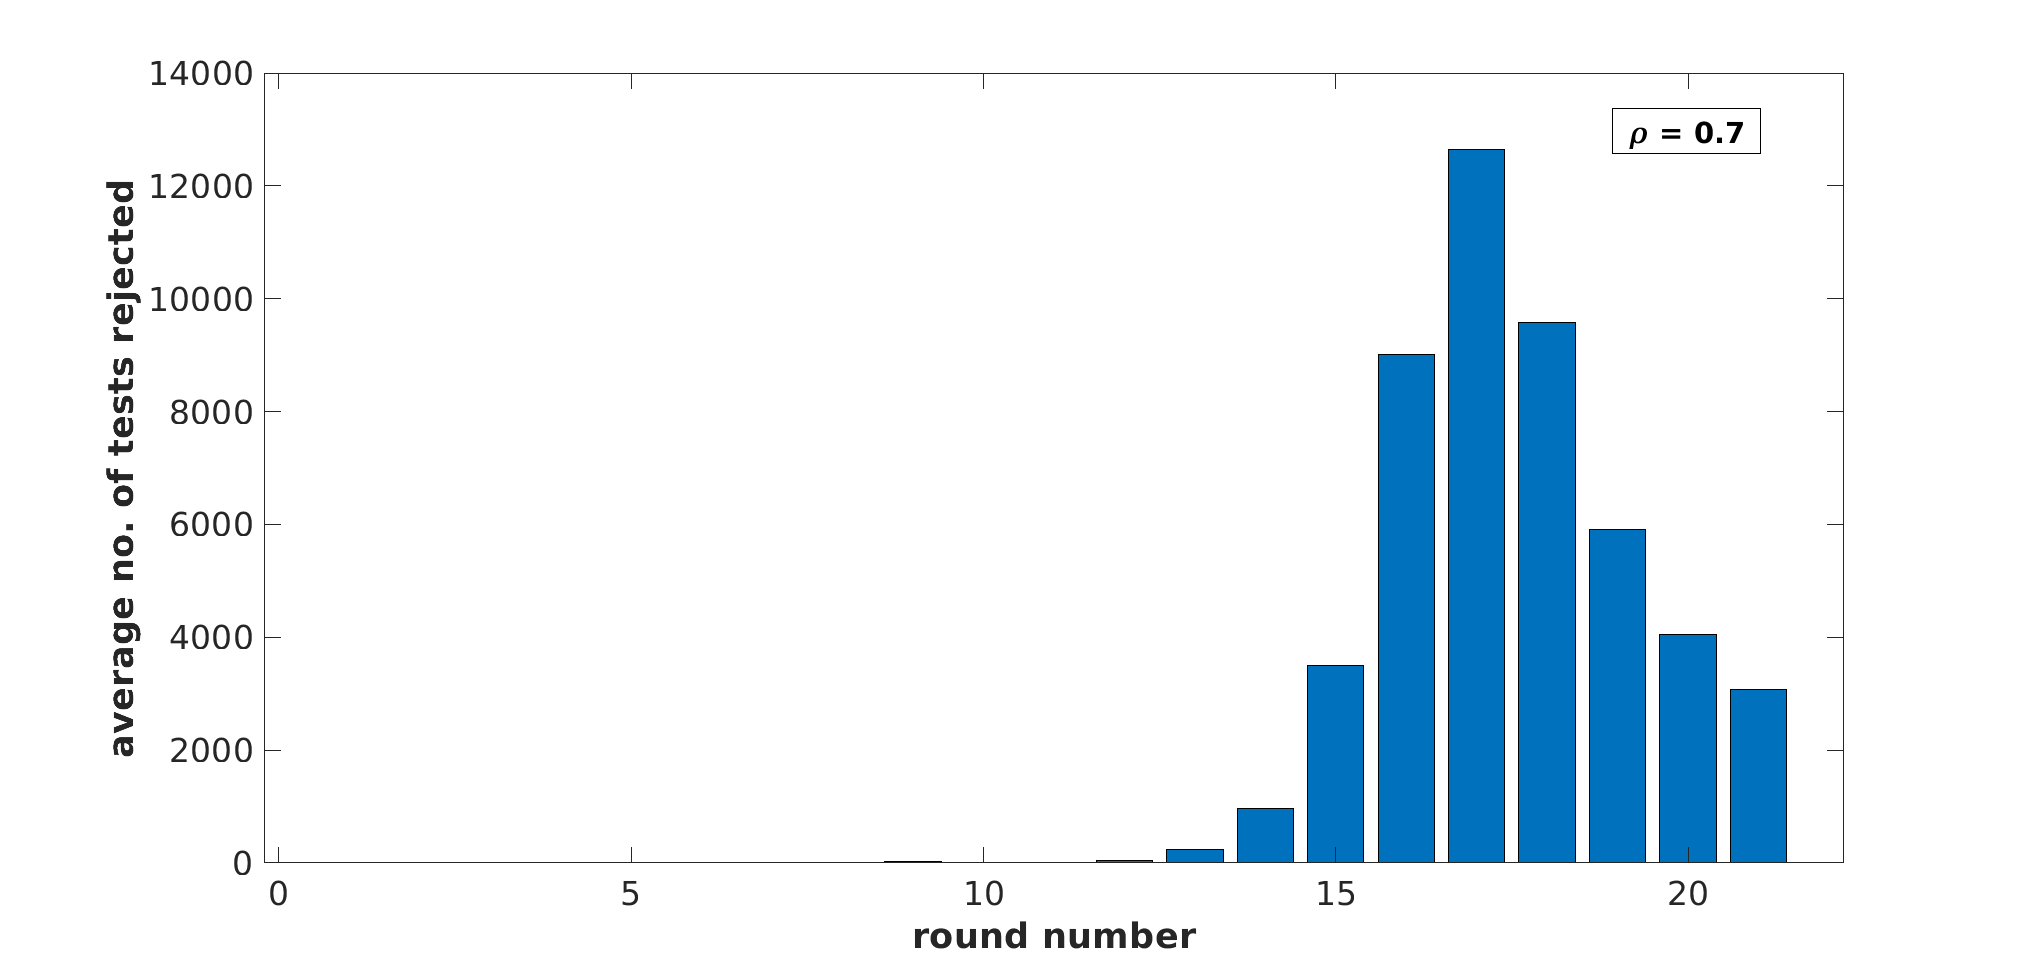
\includegraphics[scale=0.22]{figs/MIRFLICKR_1m_pruned.png}
    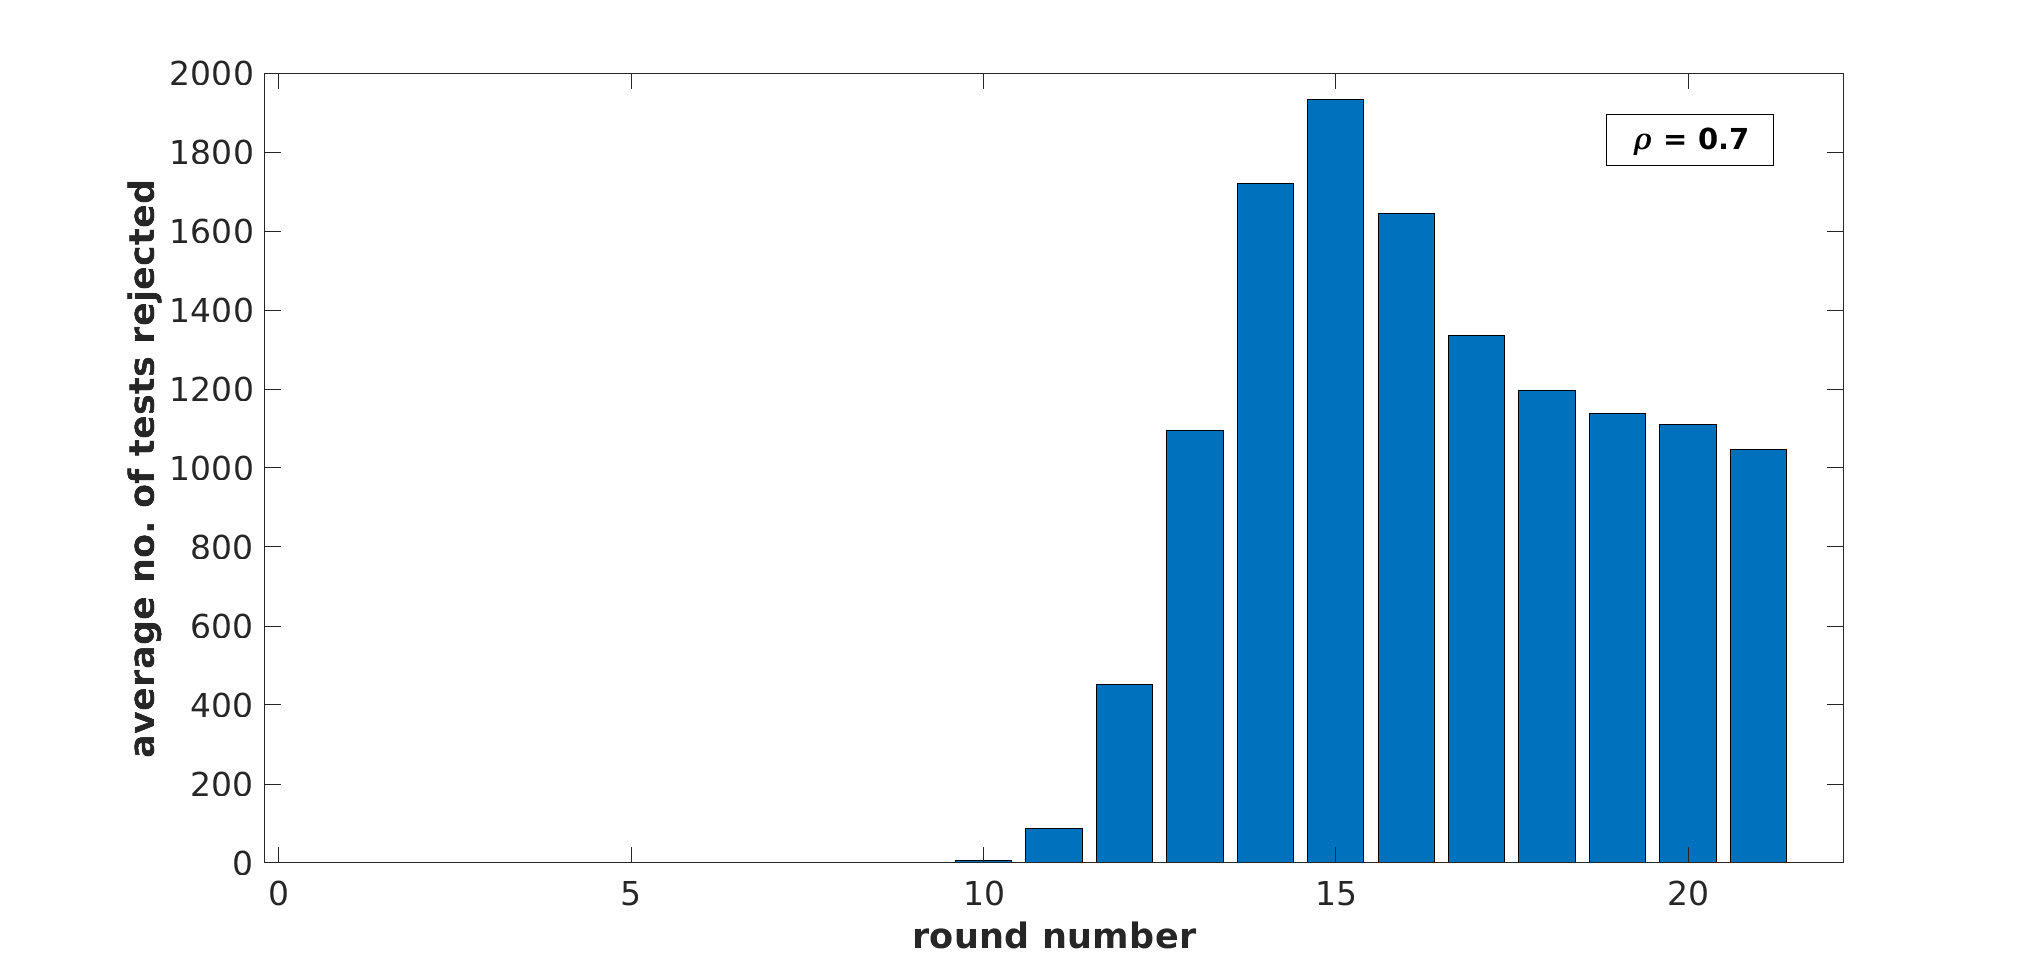
\includegraphics[scale=0.22]{figs/imageNet_pruned.png}
    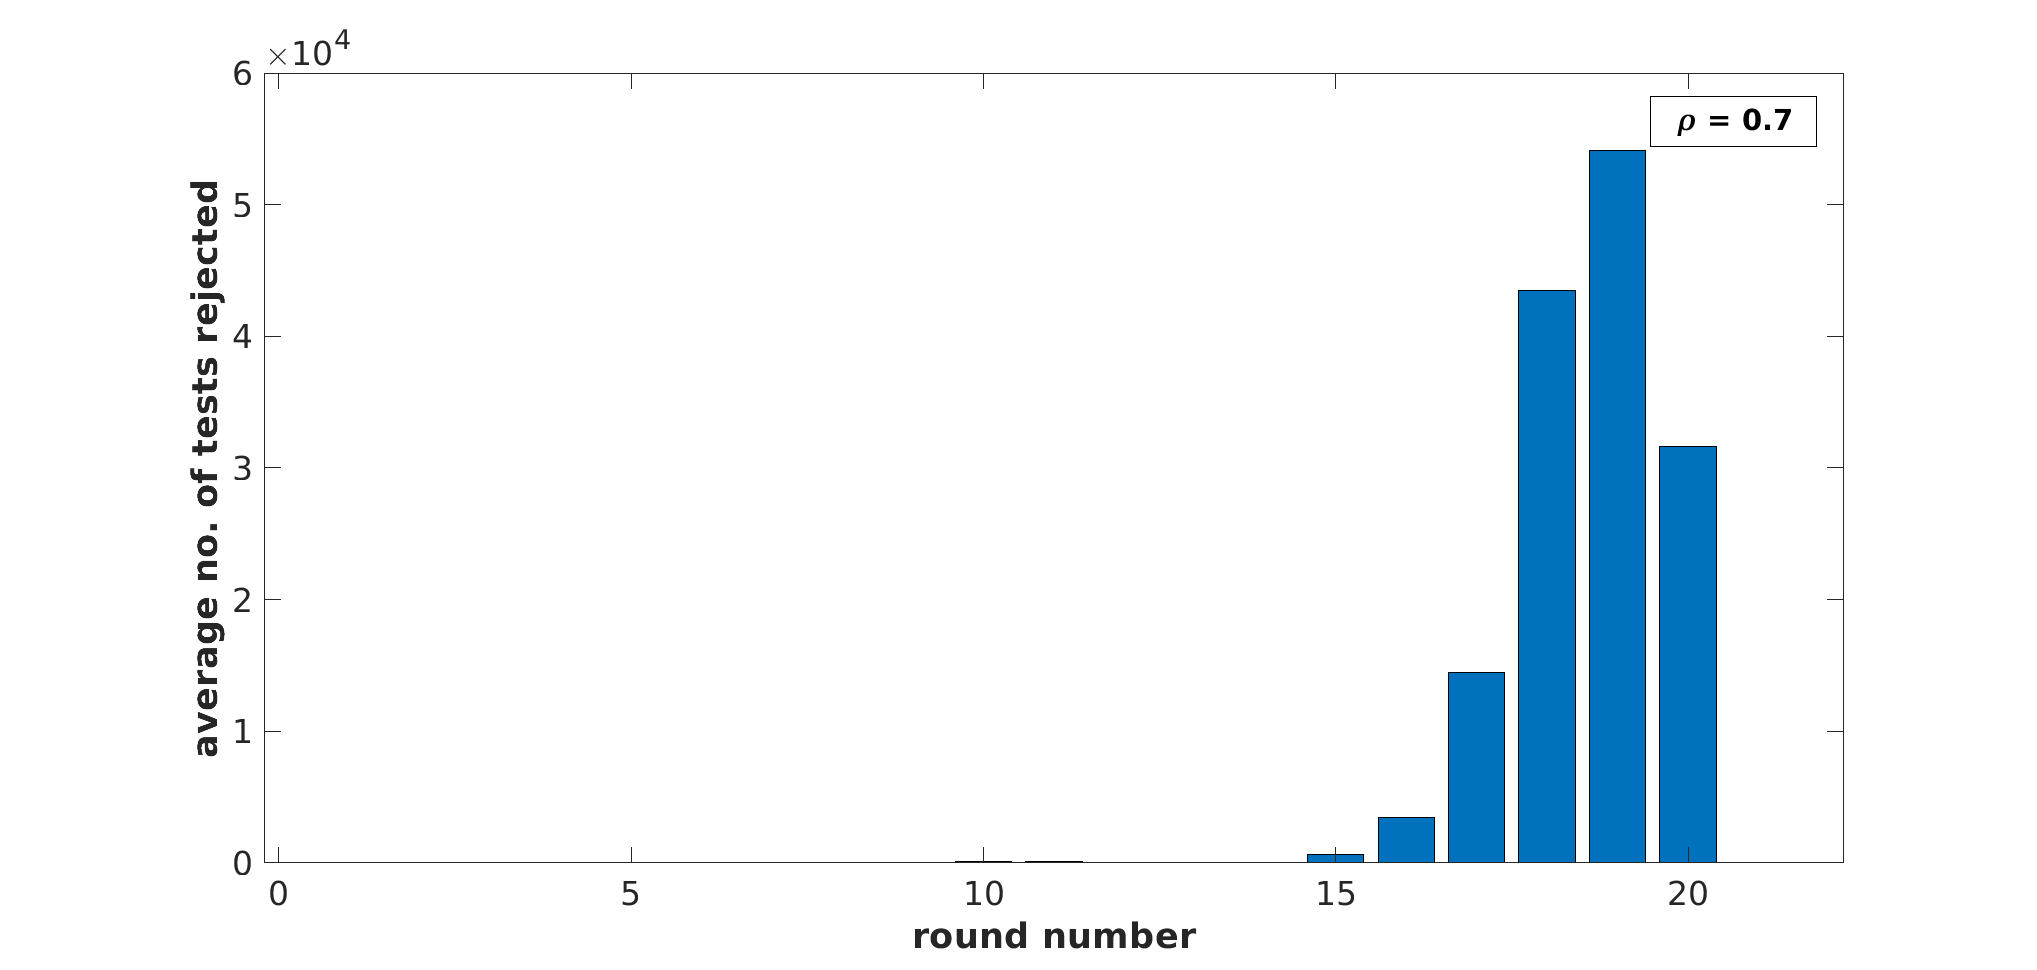
\includegraphics[scale=0.22]{figs/imdb_wiki_pruned.png}
    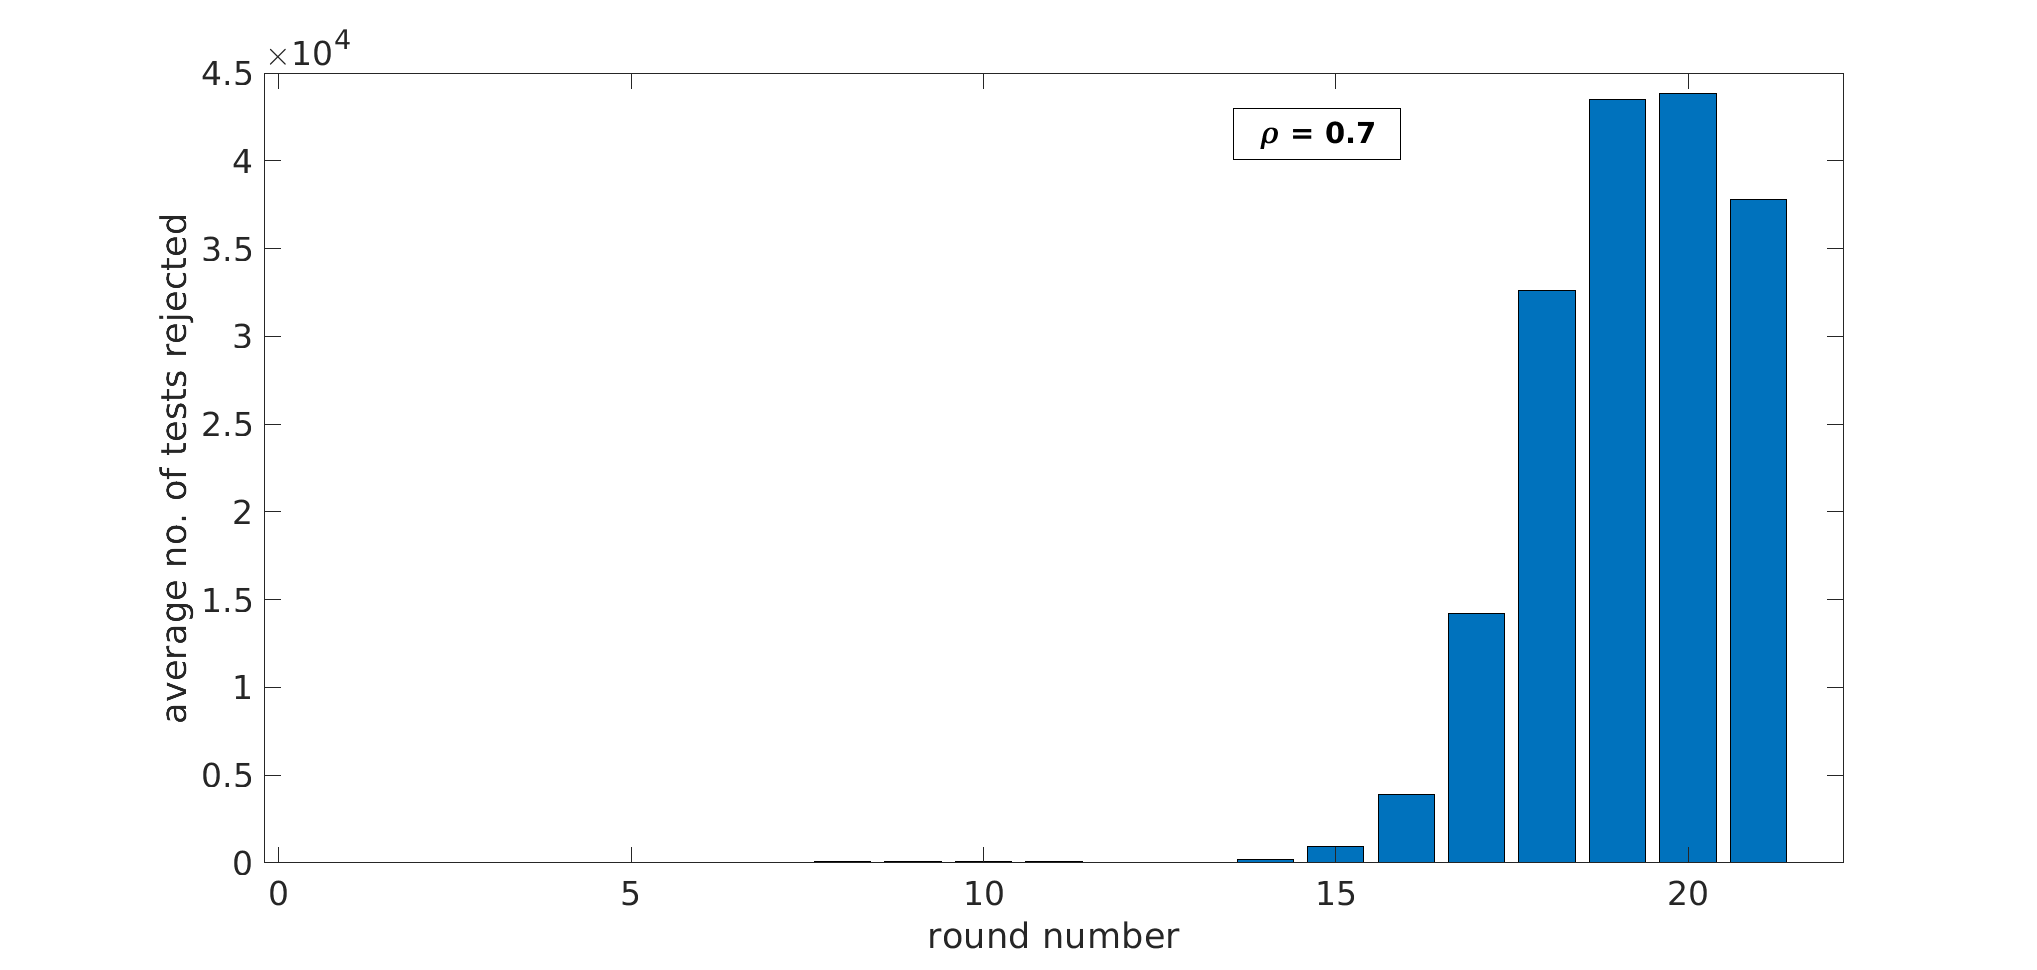
\includegraphics[scale=0.22]{figs/glami_1m_pruned.png}
    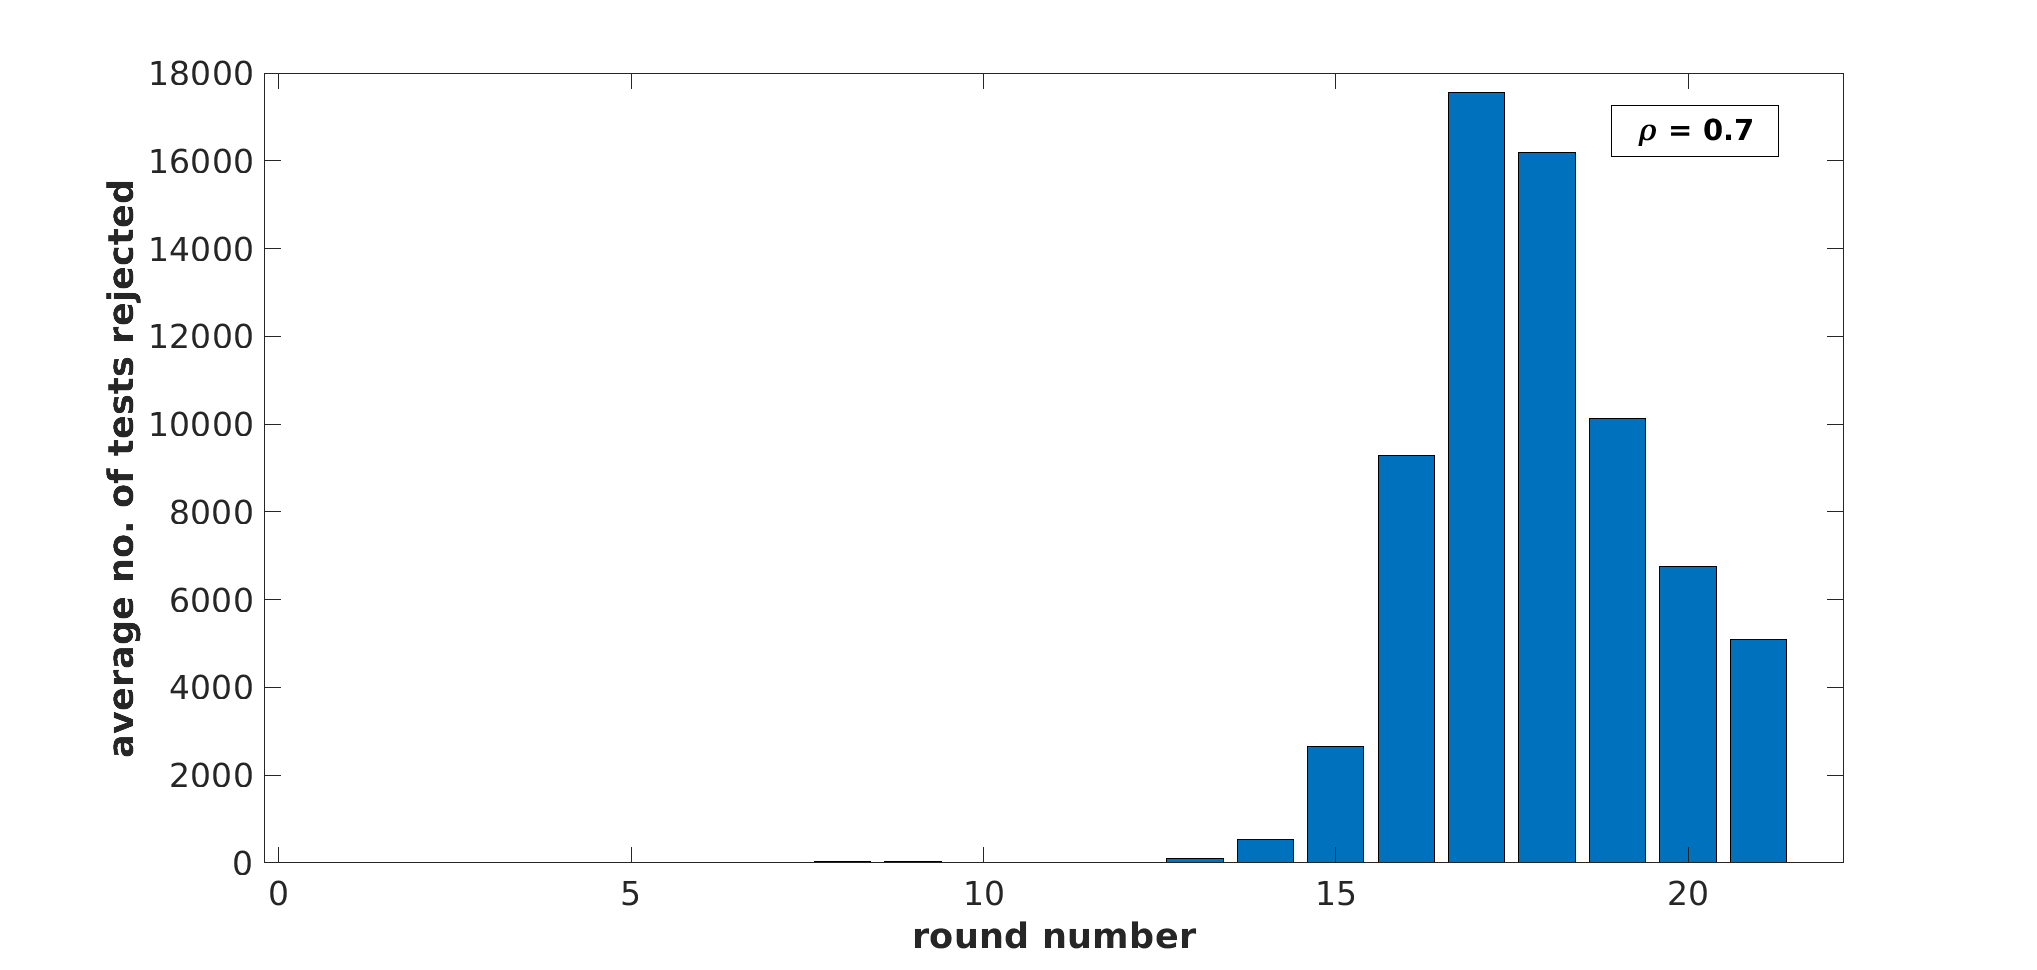
\includegraphics[scale=0.22]{figs/instaC_1m_pruned.png}
    \caption{Histograms of the number of pools rejected in every round of binary splitting for \textsf{MIRFLICKR}, \textsf{ImageNet}, \textsf{IMDB-Wiki}, \textsf{GLAMI} and \textsf{InstaCities} (left to right, top to bottom), all for $\rho \geq 0.7$.}
    \label{fig:rejection_round}
\end{figure*}

\section{Theoretical Analysis}
\label{sec:theoretical_analysis}
For the problem of binary group testing, different variants of the binary splitting approach have been shown to require just $s \log_2 N + O(s)$ or $s \log_2 (N/s) + O(s)$ tests, depending on some implementation details \cite[Theorems 1.2 and 1.3]{Aldridge2019}. Here $s$ stands for the number of defectives out of $N$. However in binary group testing, a positive result on a pool necessarily implies that at least one of the participants was defective. In our application for NN search, a pool $\boldsymbol{y}$ can produce $\boldsymbol{q}^t \boldsymbol{y} \geq \rho$ for query vector $\boldsymbol{q}$, even if \emph{none} of the vectors that contributed to $\boldsymbol{y}$ produce a dot product with $\boldsymbol{q}$ that exceeds or equals $\rho$. Due to this important difference, the analysis from \cite{Aldridge2019} does not apply in our situation. Furthermore, it is difficult to pin down a precise \emph{deterministic} number of tests in our technique. Instead, we resort to a distributional assumption on each dot product $\boldsymbol{q}^t \boldsymbol{f_i}$. We assume that these dot products are independently distributed as per a truncated normalized exponential (TNE) distribution:
\begin{equation}
p(x; \lambda) = 
\begin{cases}
\dfrac{\lambda e^{-\lambda x}}{1-e^{-\lambda}}, \textrm{ for } 0 \leq x \leq 1. \\
0, \textrm{ otherwise.}
\end{cases}
\label{eq:TNE}
\end{equation}
This distribution is obtained by truncating the well-known exponential distribution to the $[0,1]$ range and normalizing it so that it integrates to one. Larger the value of $\lambda$, the more rapid is the `decay' in the probability of dot product values from 0 towards 1. Our empirical studies show that this is a reasonable model for dot product values commonly encountered in queries in image retrieval, as can be seen in Fig.~\ref{fig:exponential} for all datasets we experimented with. Also, the best-fit $\lambda$ values are presented in the last column of Table~\ref{tab:dotproducts_stats} for different datasets. The TNE model fit may not be perfect, but less than perfect adherence to the TNE model does not change the key message that will be conveyed in this section.
\begin{figure*}
    \centering
    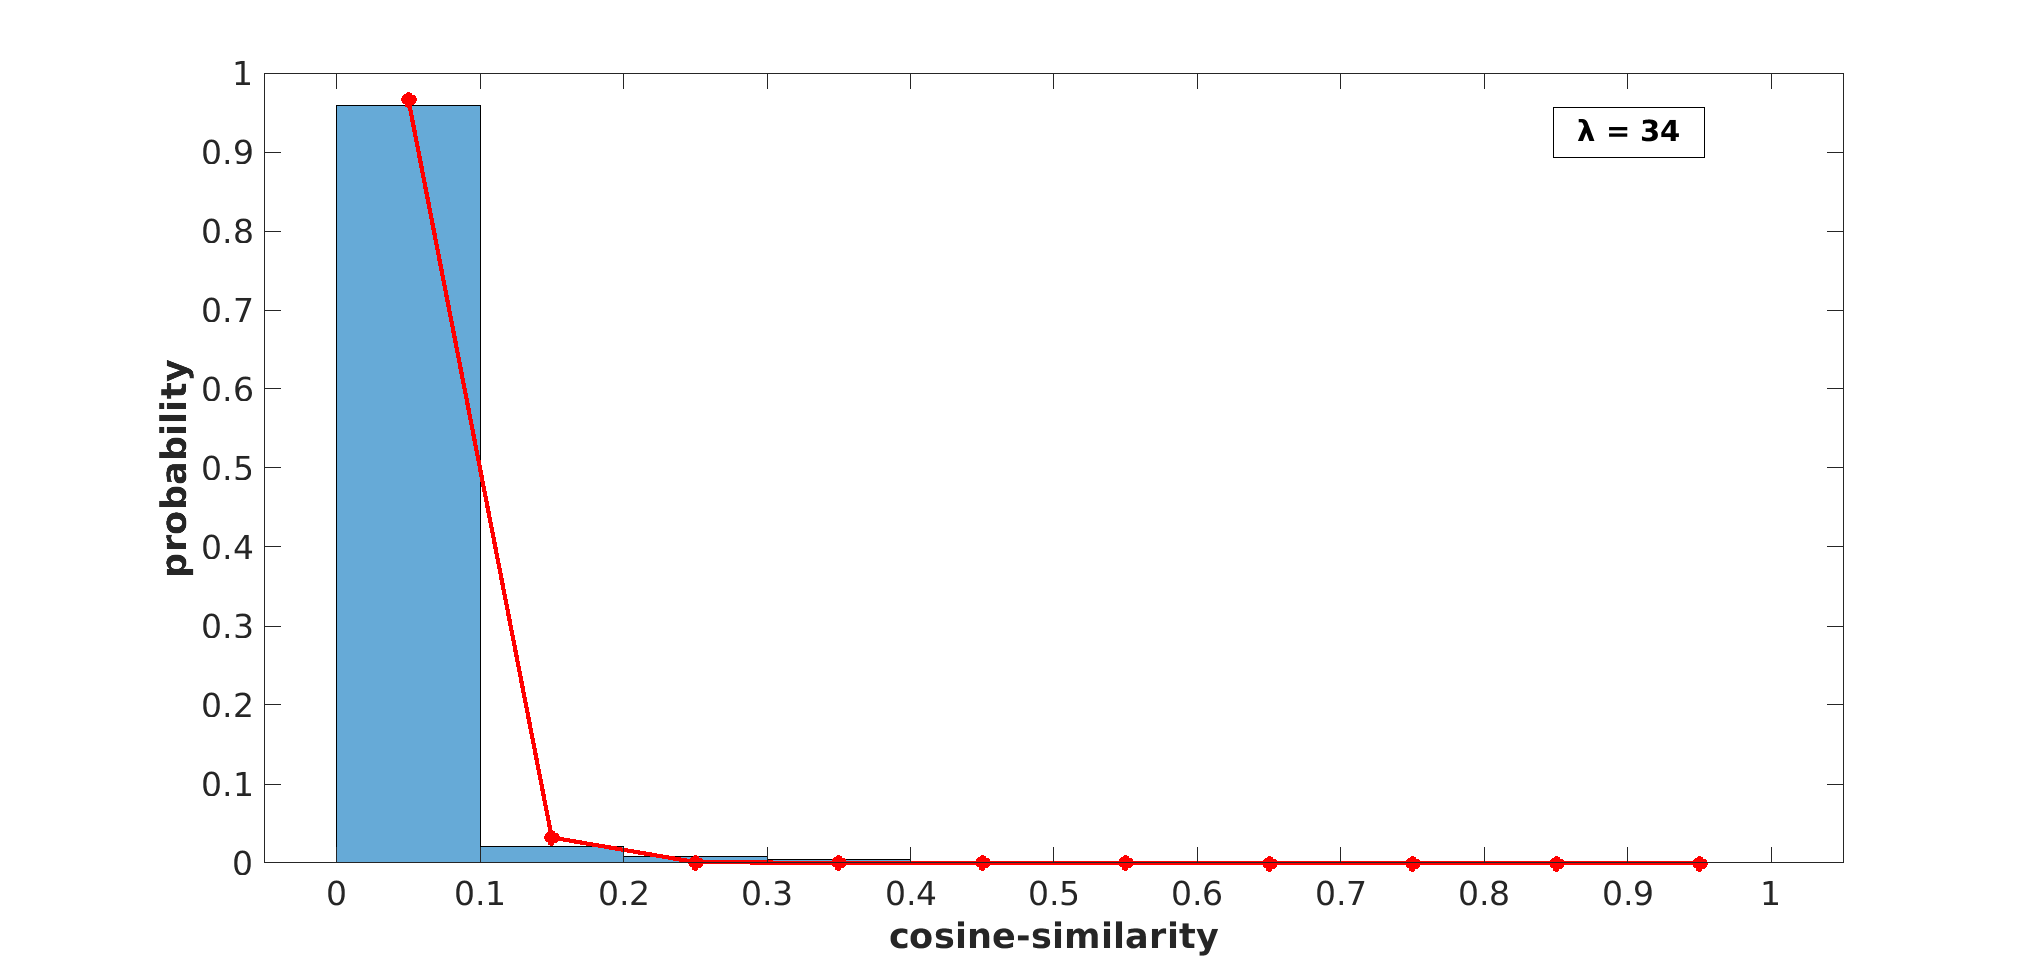
\includegraphics[scale=0.22]{figs/exp_MIRFLICKR_1m.png}
    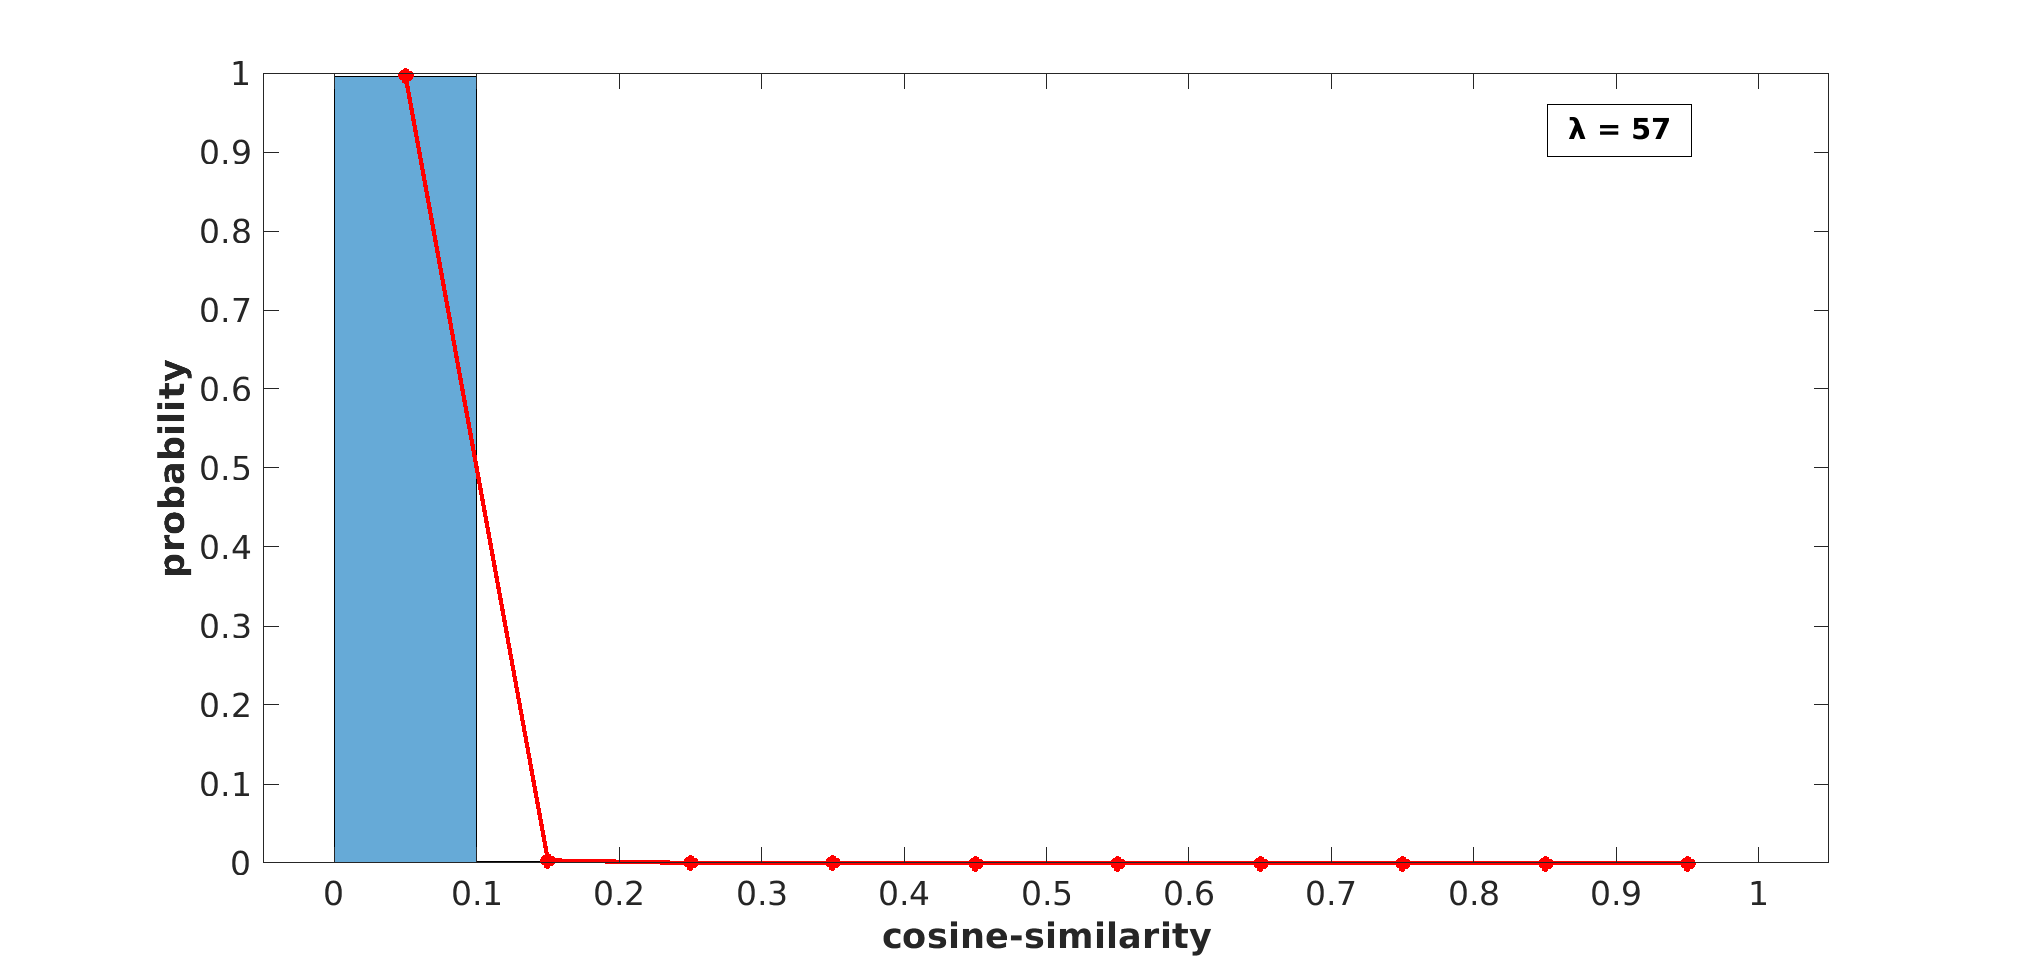
\includegraphics[scale=0.22]{figs/exp_imageNet.png}
    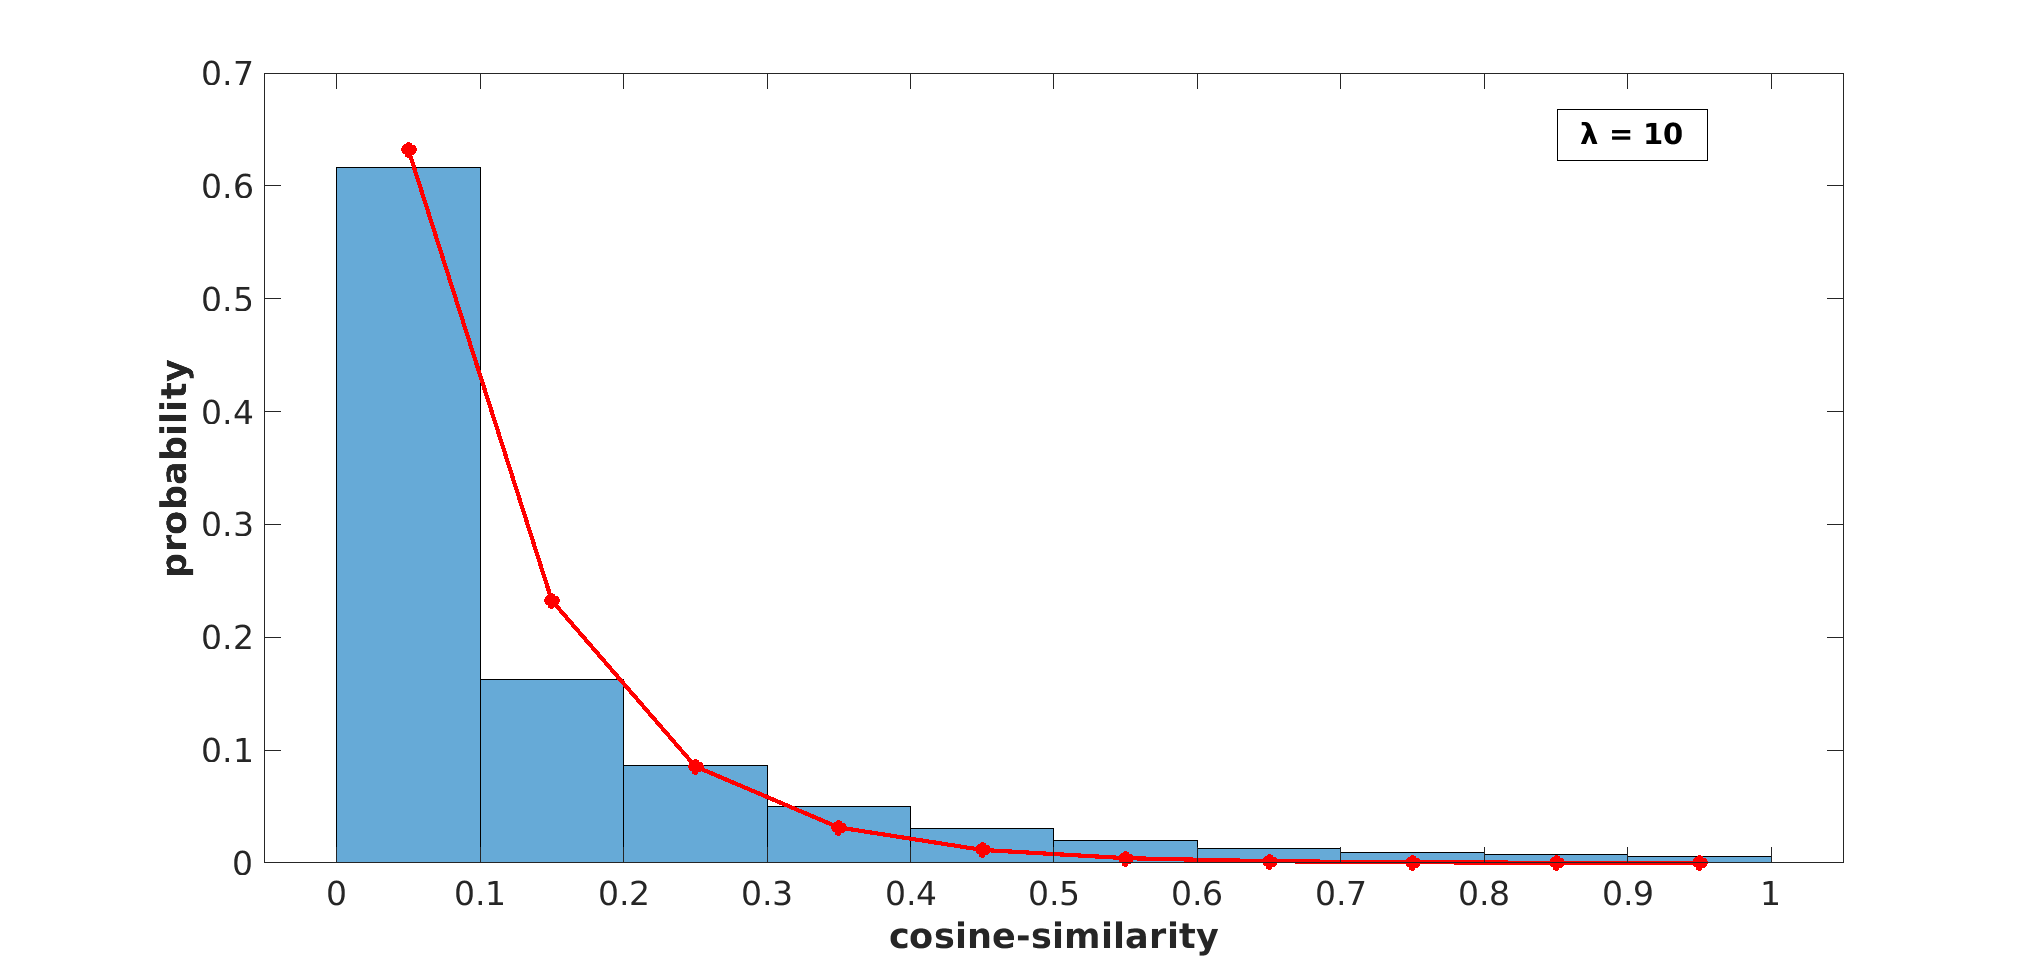
\includegraphics[scale=0.22]{figs/exp_imdb_wiki.png}
    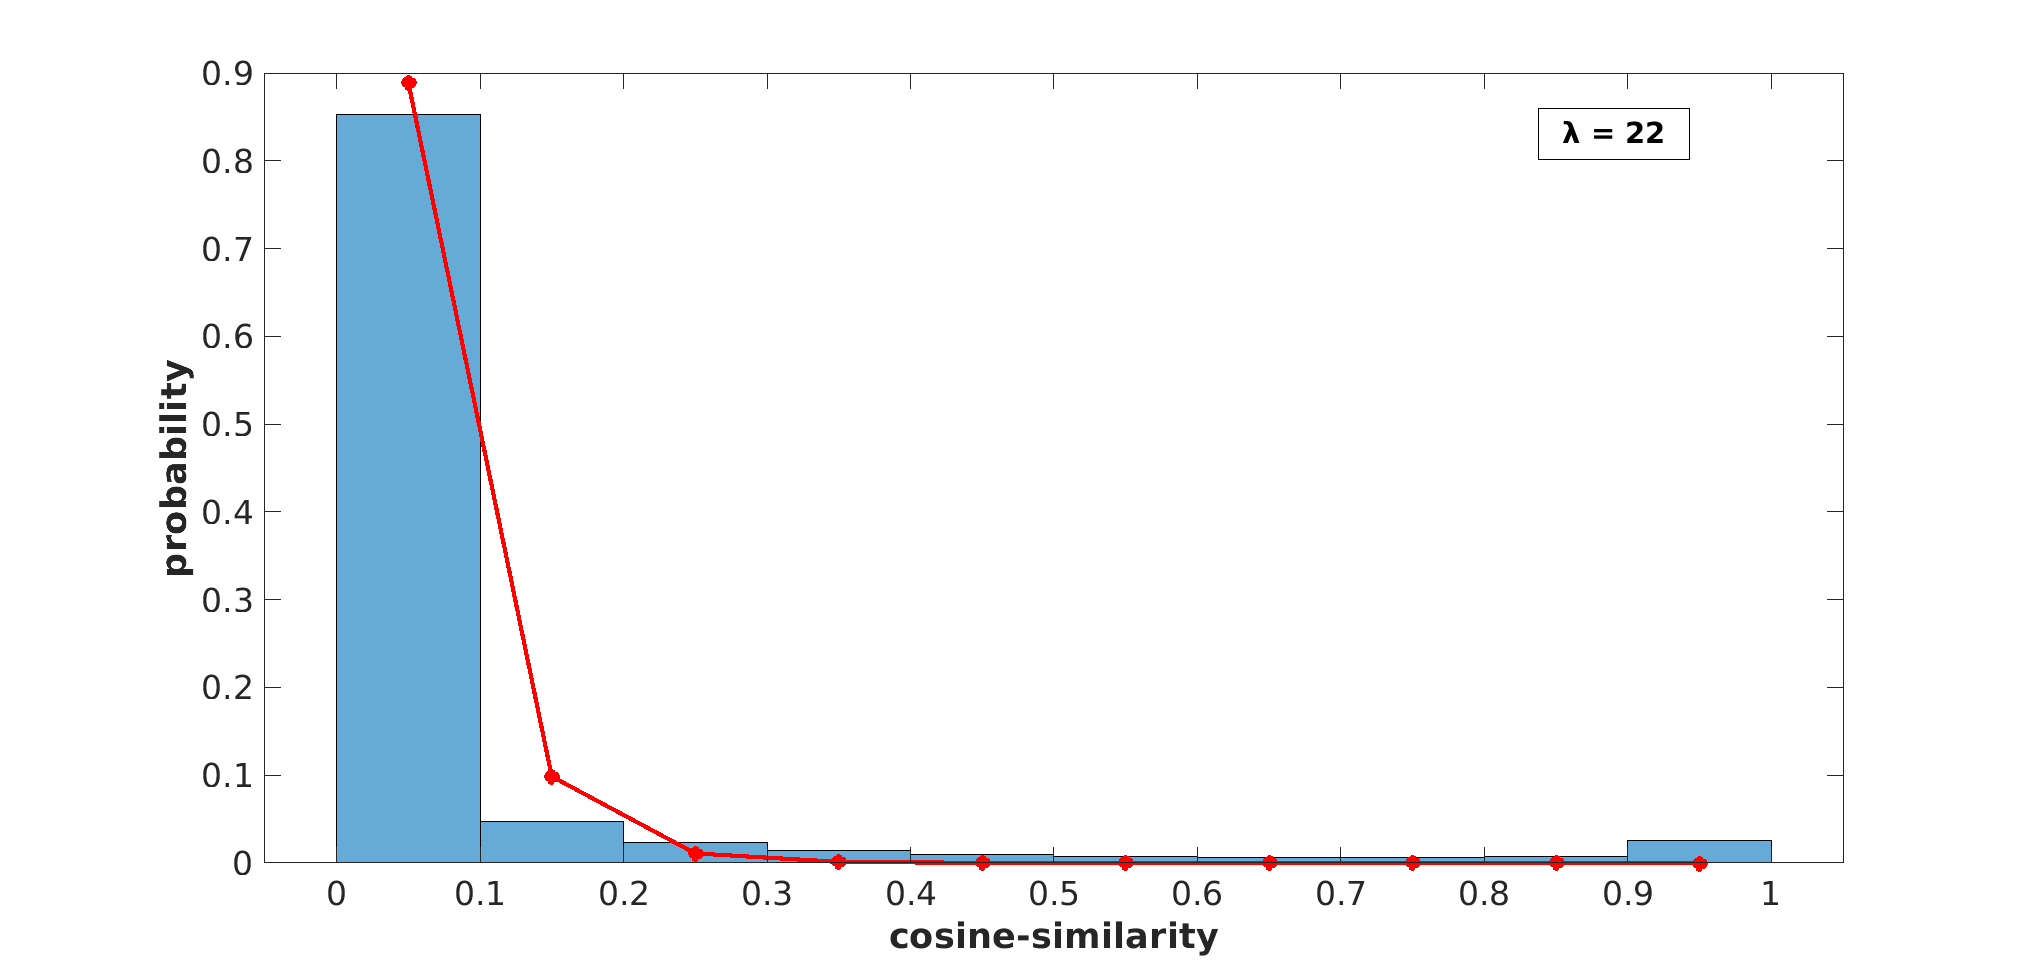
\includegraphics[scale=0.22]{figs/exp_glami_1m.png}
    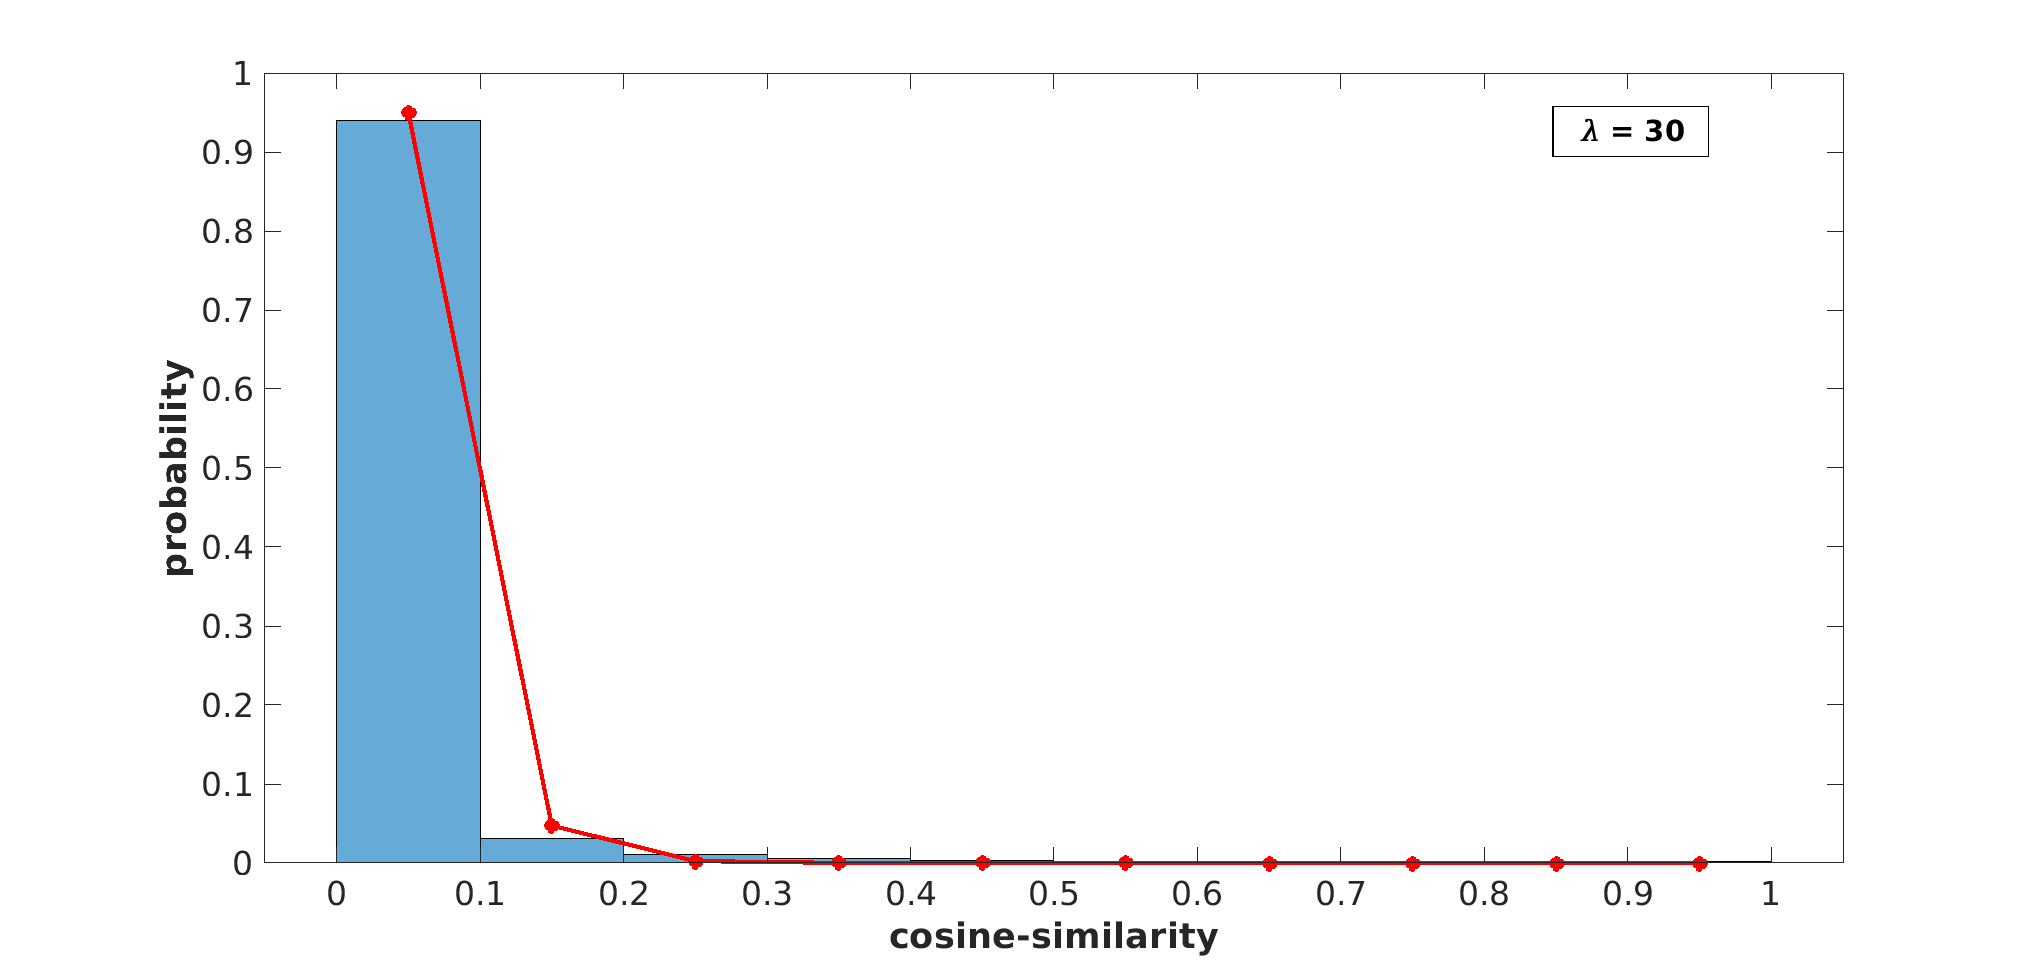
\includegraphics[scale=0.22]{figs/exp_instaC_1m.png}
    \caption{Normalized histograms (bar graphs in blue), and best-fit exponential distribution approximations (red curves), of dot products between feature vectors of query images (10,000 in number) and all gallery images of \textsf{MIRFLICKR}, \textsf{ImageNet}, \textsf{IMDB-Wiki}, \textsf{GLAMI} and \textsf{InstaCities} (left to right, top to bottom). Also see Fig. 1 of supplemental material for a plot of negative log of the histograms for clearer visualization of the smaller probability values.}
    \label{fig:exponential}
\end{figure*}
Our aim now is to determine the probability that a pool $\boldsymbol{y}$ with some $L$ participating vectors will produce a dot product value $\boldsymbol{q}^t \boldsymbol{y}$ below a threshold $\rho$. Note again that such a pool will get pruned away in binary splitting, and therefore we would like this probability to be high. Now, the $L$ individual dot-products (of $\boldsymbol{q}$ with vectors that contributed to $\boldsymbol{y}$) are independent and they are all distributed as per the TNE from Eqn.~\ref{eq:TNE}. The mean and variance of a TNE variable with parameter $\lambda$ are respectively given by 
$\left(\dfrac{1}{\lambda} + \dfrac{1}{1-e^{\lambda}}\right)$ and 
$\left(\dfrac{1}{\lambda^2} - \dfrac{e^{\lambda}}{(e^{\lambda}-1)^2}\right)$. We now apply the central limit theorem, due to which we can conclude that $\boldsymbol{q}^t \boldsymbol{y}$ is (approximately) Gaussian distributed with a mean $\mu \triangleq L\left(\dfrac{1}{\lambda} + \dfrac{1}{1-e^{\lambda}}\right)$ and variance $\sigma^2 \triangleq L\left(\dfrac{1}{\lambda^2} - \dfrac{e^{\lambda}}{(e^{\lambda}-1)^2}\right)$. With this, we can easily compute $P(\boldsymbol{q}^t \boldsymbol{y} \leq \rho)$ given a value of $L$ and $\rho$. Our numerical experiments, illustrated in Fig.~\ref{fig:prob_dotproducts}, reveal that this probability increases with $\lambda$ and decreases as $L$ increases. This tallies with intuition, and supports the hypothesis that a larger number of pools will be pruned away in a given round if there is more rapid decrease in the probability of dot product values from 0 to 1. 
\begin{figure*}
    \centering
    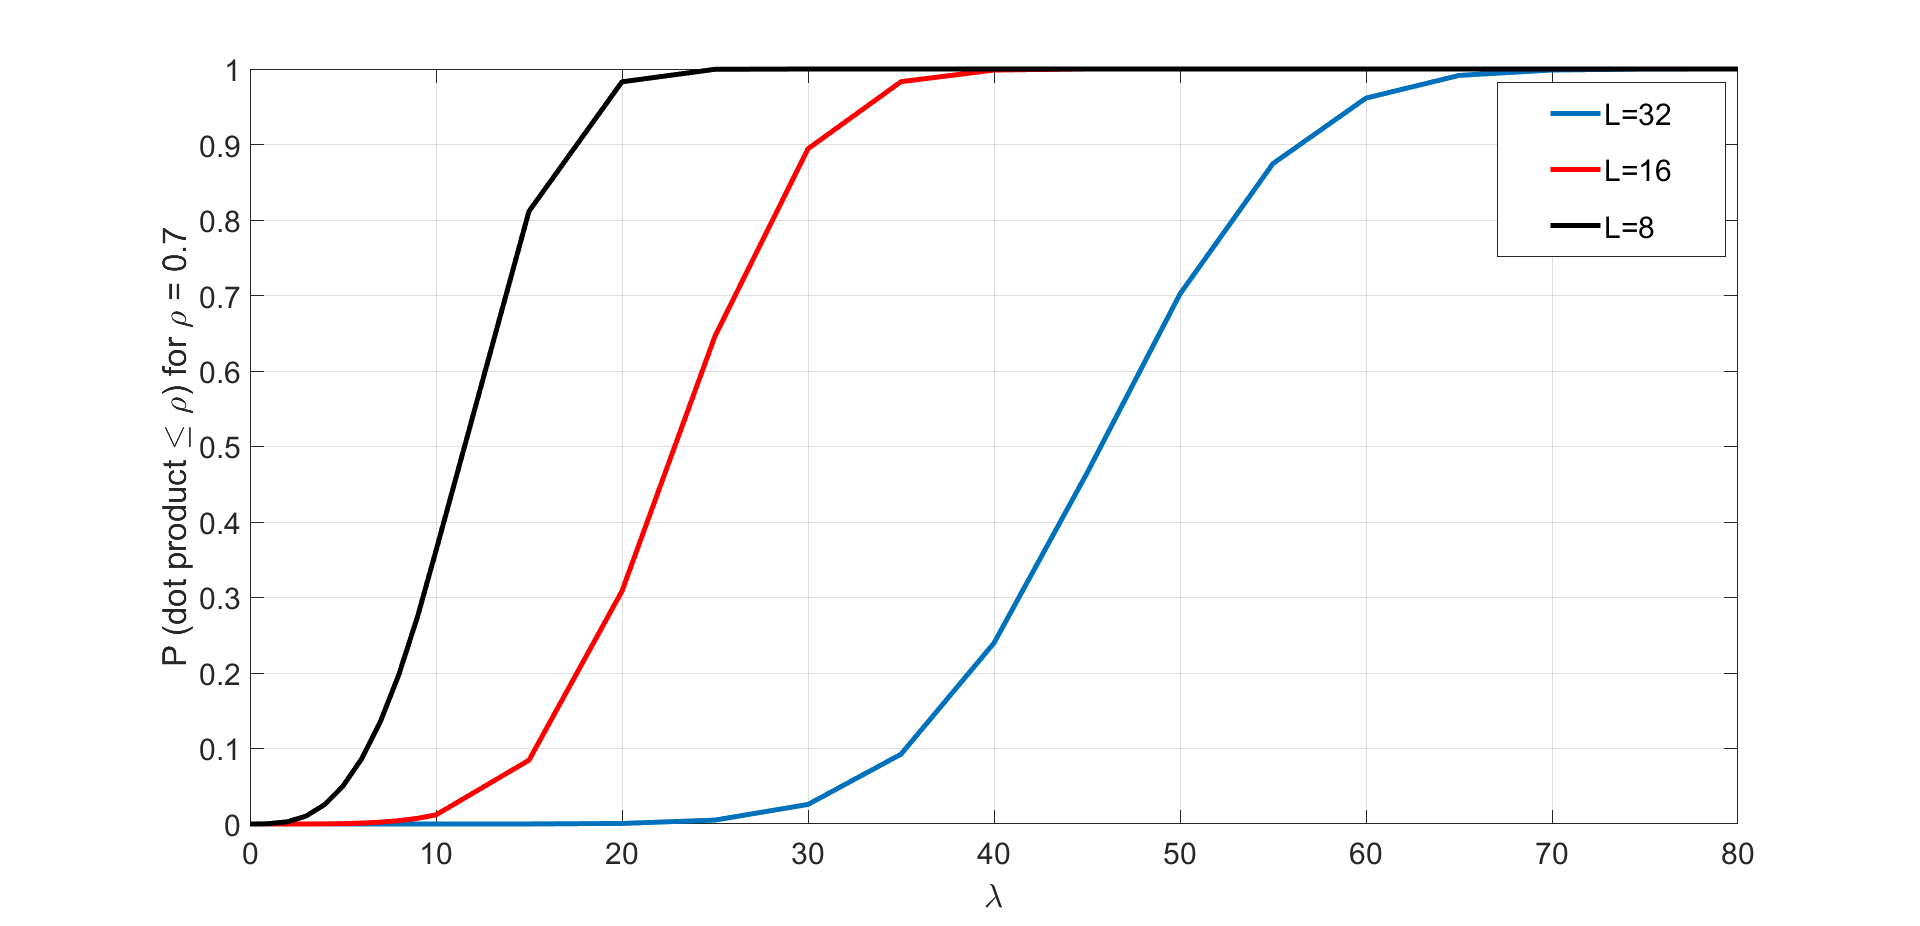
\includegraphics[scale=0.25]{figs/prob_dp.png}
    \caption{The probability that the dot product of a query vector $\boldsymbol{q}$ with a pool created from $L$ participating vectors, falls below $\rho = 0.7$, as a function of $\lambda$ for $L \in \{8,16,32\}$.}
    \label{fig:prob_dotproducts}
\end{figure*}
We are now equipped to determine the expected number of tests (dot products) to be computed per query, given such a TNE distribution for the dot products. Given a value of $\rho$, let us denote the probability that a pool with $L$ participants will get pruned away as $p_L(\rho)$. For any $L \geq 6$, this probability is computed using the TNE and CLT based method described earlier. For $L < 6$, the Gaussian distributed can be replaced by a truncated Erlang distribution, as the sum of independent exponential random variables follows an Erlang distribution. Even this case, $P(\boldsymbol{q}^t \boldsymbol{y} \leq \rho)$ increases with $\lambda$ and decreases with $L$. 

\begin{table}
\centering
\begin{tabular}{ |c|c|c|c| } 
 \hline
 \rowcolor{Gray}
Database & & &\\\hline
 \rowcolor{Gray}
\textsf{MIRFLICKR}, $N=1M$ & $\rho = 0.7$ & $\rho = 0.8$ & $\rho = 0.9$\\\hline
Empirical & 51690 &	44194 &	37788 \\
Theoretical &	63838 & 	57553	& 50094 \\ \hline
 \rowcolor{Gray}
\textsf{ImageNet}, $N = 1M$ & $\rho = 0.7$ & $\rho = 0.8$ & $\rho = 0.9$\\\hline
Empirical &	13852	& 12339 & 	10801\\ 
Theoretical	& 34524	& 32603	& 31345\\\hline
 \rowcolor{Gray}
\textsf{IMDB-Wiki}, $N = 500K$ & $\rho = 0.7$ & $\rho = 0.8$ & $\rho = 0.9$\\\hline			
Empirical &	160020 &	141290 &	125050\\
Theoretical &	113600 &	99552	& 87835\\\hline
 \rowcolor{Gray}
\textsf{GLAMI}, $N = 1M$ & $\rho = 0.7$ & $\rho = 0.8$ & $\rho = 0.9$\\\hline	
Empirical &	215630 &	197200 &	178700\\
Theoretical &	95633 &	81417 &	71343\\\hline		
 \rowcolor{Gray}
\textsf{InstaCities}, $N = 1M$	& $\rho = 0.7$ & $\rho = 0.8$ & $\rho = 0.9$\\\hline
Empirical &	72729 &	62741	& 54125\\
Theoretical &	71021 & 	63453 &	57944\\\hline
\end{tabular}
\caption{Empirically observed average and theoretically predicted expected number of dot products (Eqn.~\ref{eq:E_rho}) for queries with $\rho \in \{0.7,0.8,0.9\}$ for different datasets. See explanation at the end of Sec.~\ref{sec:theoretical_analysis}.}
\label{tab:emp_theor}
\end{table}

In round 1, there is only one pool and it contains all $N$ vectors. It will get pruned away with probability $p_N(\rho)$, for a given fixed threshold $\rho$ and fixed $\lambda$. The expected number of pools in round 2 will be $Q_2 \triangleq 2(1-p_N(\rho))$, each of which will be pruned away with probability $p_{N/2}(\rho)$. The factor 2 is because each pool gets split into two before sending it to the next round of binary splitting. The expected number of pools in round 3 will be $Q_3 \triangleq 2(1-p_{N/2}(\rho))Q_2$. Likewise, in the $k$th round, the expected number of pools is $Q_k = 2(1-p_{N/2^{k-2}}(\rho))Q_{k-1}$. Hence the expected number of tests per query in our approach will be:
\begin{equation}
E(\rho) \triangleq 1+\frac{1}{2}\sum\limits_{i=2}^{\lceil \log_2 N +1 \rceil} Q_i.
\label{eq:E_rho}
\end{equation}
This is because there are at most $\lceil \log_2 N +1 \rceil$ rounds. The factor $\frac{1}{2}$ is due to the fact that the number of tests is always half the number of pools (see second para. of Sec.~\ref{sec:method}).
The value of $E(\rho)$ decreases with $\lambda$ as $p_N(\rho), p_{N/2}(\rho),...,p_{N/2^{k-2}}(\rho)$ all increase with $\lambda$. Our theoretical analysis depends on $\lambda$, but note that our algorithm is completely agnostic to $\lambda$ and does not use it in any manner. For values of $\rho \in \{0.7,0.8,0.9\}$, we compared the theoretically predicted average number of dot products from Eqn.~\ref{eq:E_rho} to the experimentally observed number for all datasets. These are presented in Tab.~\ref{tab:emp_theor}, where we observe that for \textsf{MIRFLICKR}, \textsf{ImageNet} and \textsf{InstaCities}, the theoretical number is generally \emph{greater} than the empirical number. This is because the dot products for these datasets decay slightly faster than what is predicted by an exponential distribution, as can be seen in Fig.~\ref{fig:exponential}. On the other hand, for \textsf{IMDB-Wiki} and \textsf{GLAMI}, the theoretical number is \emph{less} than the empirical number because the dot products decay slower for these datasets than what is predicted by an exponential distribution. In particular, for \textsf{GLAMI}, we observe that the $[0.9,1]$ bin contains more entries than what is predicted by an exponential distribution. 

\section{Conclusion}
\label{sec:conclusion}
We have presented a simple and intuitive multi-round group testing approach for nearest neighbor search. Our method outperforms exhaustive search by a large factor in terms of query time without losing accuracy, on datasets where query vectors are dissimilar to the vast majority of vectors in the gallery. The larger the percentage of dissimilar vectors, the greater is the speedup our algorithm will produce. Our technique has no tunable parameters. It is also easily applicable to situations where new vectors are dynamically added to an existing gallery, without requiring any expensive updates. Apart from this, our technique also has advantages in terms of accuracy of query results over some recent, state of the art methods from the literature. At present, a pool may produce a large dot product value with a query vector, even though many or even all the members of the pool are dissimilar to the query vector. Developing techniques to reduce the frequency of such situations, possibly using various hashing techniques, is an important avenue for future work. Another avenue is to explore the applications of this technique in efficient high dimensional probability density estimation.

\bibliographystyle{ACM-Reference-Format}
\bibliography{sample-base}

\end{document}
\endinput
%%
%% End of file `sample-authordraft.tex'.
